\chapter{Fundamentos}
\label{cha:fundamentos}

Neste capítulo é apresentada a revisão bibliográfica para a fundamentação do trabalho.

Seis conceitos básicos são apresentados: ``Indústria 4.0'', ``Logística \& Cadeia de Suprimentos'', ``Ciclo de vida do produto'', ``Memória digital do produto'', ``Arquitetura orientada a serviços'' e ``Modelagem de sistemas''.

A inter-relação entre esses conceitos é a base para o entendimento e desenvolvimento da arquitetura e para o estudo das implicações do compartilhamento de informações no ciclo de vida do produto no contexto da I4.0.

\section{Indústria 4.0 (I4.0)}
\label{sec:industria4}

I4.0 é o nome dado às recentes inovações em relação às tecnologias utilizadas em processos industriais e à forma de organização dos sistemas industriais. Tais tecnologias são inseridas com o propósito de se oferecer um alto nível de automação e intercâmbio de informações entre equipamentos e produtos \cite{lasi2014industryfour}.

O nome I4.0 se dá ao fato de ser considerada a quarta revolução com relação às tecnologias de produção industrial, sendo as ``revoluções industriais'' consideradas evoluções tecnológicas que levaram a mudanças significativas na forma de produção da época. As outras transições dentro da indústria ao longo da história aconteceram: no campo da mecanização da produção (1\textsuperscript{a} revolução industrial), com a produção em massa e intenso uso de energia elétrica (2\textsuperscript{a} revolução industrial) e com a expansão da automação e eletrônica (3\textsuperscript{a} revolução industrial) \cite{lasi2014industryfour}. Tal histórico de revoluções no campo da indústria é ilustrado na \autoref{fig:i4-2}.

\begin{figure}[htb]
	\centering
	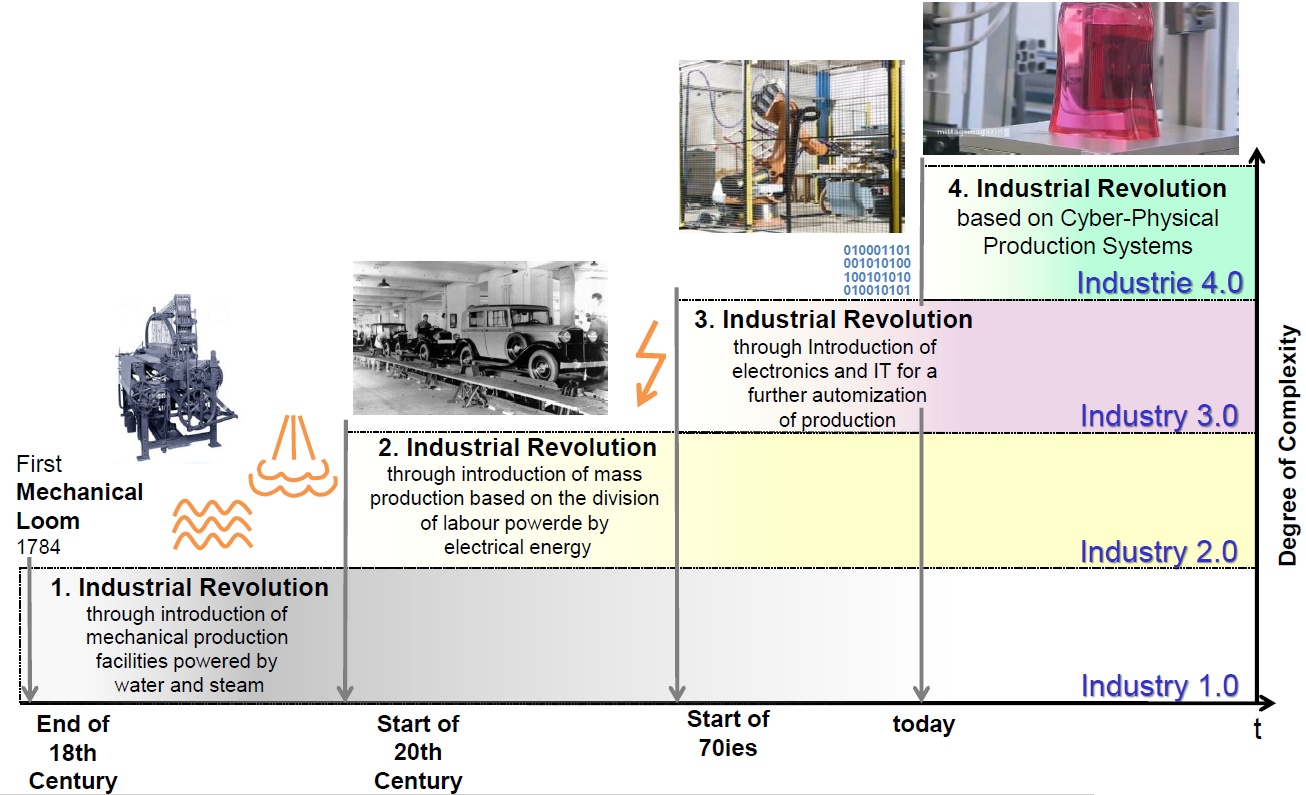
\includegraphics[width=1\textwidth]{i4-2.png}
	\caption{Evolução da indústria por meio das revoluções industriais.}
	\label{fig:i4-2}
	\fonte{\citeonline{wahlster2013industrie} (adaptado).}
\end{figure}

O termo I4.0 foi trazido a público pela primeira vez em 2011 na feira industrial de Hanôver (\textit{Hannover-Messe}) \cite{kagermann2011industrie}, que é uma feira tecnológica de relevância internacional e visa apresentar inovações relacionadas ao setor industrial.

Por vezes, a I4.0 é tratada também como a convergência da produção industrial com as novas Tecnologias de Informação e Comunicação (TIC) \cite{hermann2016design}.

Embora o termo I4.0 seja bastante comum na discussão tecnológica atual, muitas empresas, centros de pesquisa e universidades não mantêm uma definição comum sobre o assunto. Segundo \citeonline{hermann2016design} e com base em uma revisão de literatura feita pelos mesmos autores, a I4.0 é composta por quatro princípios, conforme listados na \autoref{tab:principios-i4}.

\begin{table}[htb]
	\centering
	\footnotesize
	\caption{Princípios para implantação da I4.0 baseados em \citeonline{hermann2016design}.}
	\label{tab:principios-i4}
	\begin{tabular}{p{3cm}p{12cm}}
		\hline
		\textbf{Princípio}           & \textbf{Descrição}                                                                                                                                                                                                                                                                                                              \\

		\hline
		Interoperabilidade           &
		Capacidade das coisas (ativos, máquinas, dispositivos, sensores, pessoas, etc) de comunicarem entre si dentro de um sistema por meio de padrões definidos.                                                                                                                                                                                                     \\

		\hline
		Transparência de informação  &
		Tornar acessíveis informações úteis para os demais ativos conectados à rede. Informações do mundo digital como documentos eletrônicos, desenhos, modelos de simulação. E informações sobre o mundo real, como posição, dados de sensores de temperatura, vibração, etc.                                                                                        \\

		\hline
		Descentralização de decisões &
		Permitir a tomada de decisões baseada nas informações coletadas pelo próprio ativo e dar a ele autonomia para decidir qual será sua próxima função/operação. Desta forma, um planejamento ou controle central de processos produtivos não se faz essencial e o sistema de produção se torna menos hierarquizado.                                               \\

		\hline
		Assistência técnica          &
		Devido à complexidade da produção, com redes complexas e tomada de decisões descentralizadas, os seres humanos precisam ser auxiliados por sistemas de assistência de forma a dar compreensibilidade ao processo e às tomadas de decisão necessárias. Os sistemas de assistência devem agregar e tornar visualizáveis as informações de maneira compreensível. \\

		\hline
	\end{tabular}
\end{table}

Esta nova revolução industrial já está em curso, segundo o Fórum Econômico Mundial \cite{schwab2016fourth} em seu encontro anual realizado em Davos no ano de 2016, e as razões para o surgimento desse novo paradigma de produção incluem: a competição acirrada entre empresas, a alta complexidade de manufatura dos produtos e os seus altos níveis de personalização por parte dos clientes \cite{bordeleau2018bi, vaidya2018industryfour}.

Uma das bases para esse novo paradigma de produção é a interconexão entre ``coisas'' no ambiente de produção por meio de identificadores individuais usando conceitos de Internet das Coisas (\textit{Internet of Things} - IoT) e de Internet das Coisas Industrial (\textit{Industrial Internet of Things} - IIoT). Tais ``coisas'' se referem a equipamentos, produtos, máquinas, peças, pessoas e quaisquer outros elementos envolvidos no ambiente industrial, que por vezes também são denominados ``ativos''.

Esses ativos são inseridos no meio digital, onde podem trocar informações e executar funções sobre seus correspondentes reais de forma mais autônoma e com menor intervenção humana por meio do uso extensivo de recursos avançados de tecnologias da informação e comunicação \cite{adolph2018roadmap}. Devido a essa maior interação entre ativos no sistema de fabricação, extingue-se a relação essencialmente hierarquizada de gestão e controle da indústria tradicional e, assim, estes ativos passam a deter a capacidade de se comunicarem diretamente uns com outros, conforme ilustrado na \autoref{fig:i3-to-i4}.

\begin{figure}[htb]
	\centering
	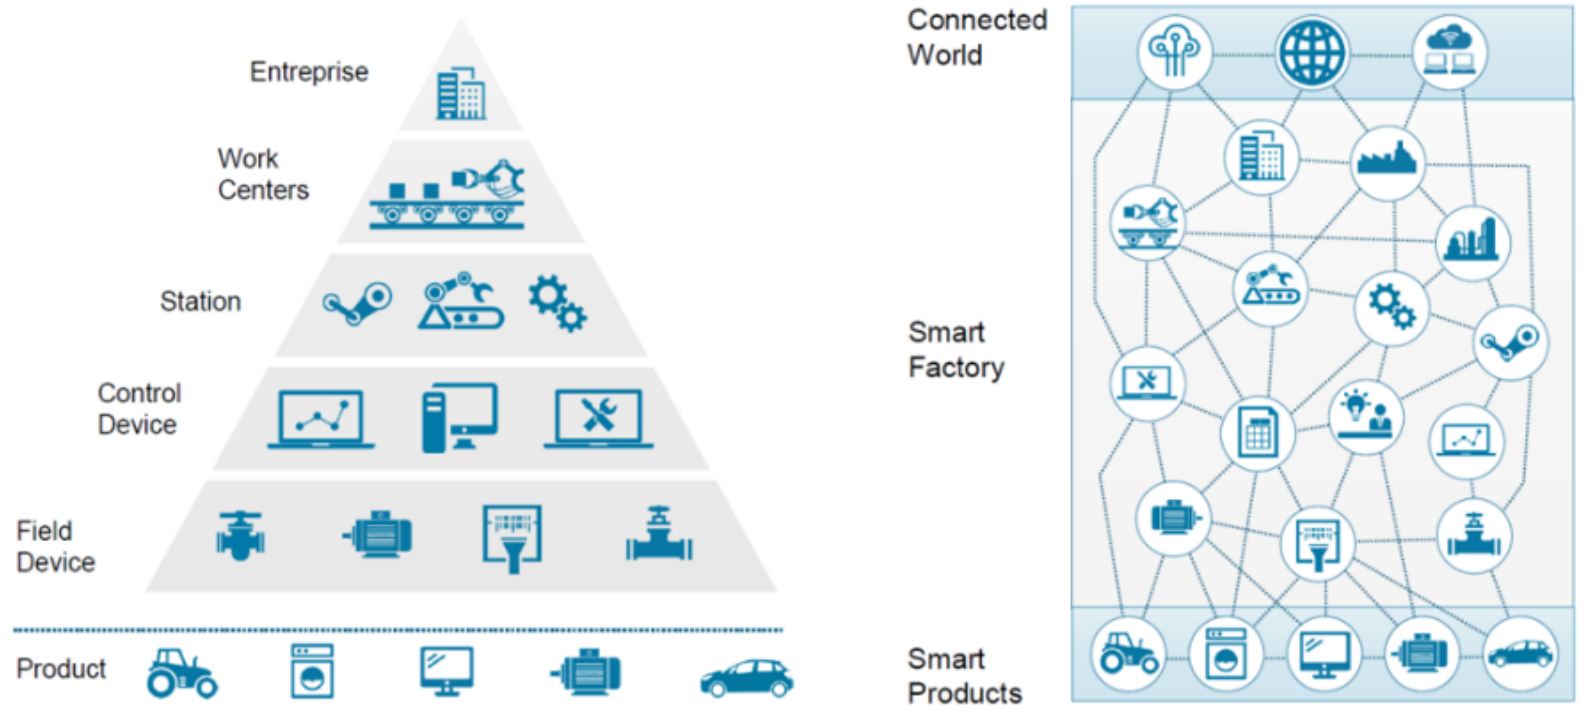
\includegraphics[width=1\textwidth]{i3-to-i4.png}
	\caption{Transição do (a) modelo hierárquico tradicional de gestão e controle para o (b) modelo flexível de comunicação entre dispositivos na I4.0.}
	\label{fig:i3-to-i4}
	\fonte{\citeonline{schmittner2017mtom} (adaptado).}
\end{figure}

Essa automatização dos ativos tem potencial para dar mais eficiência aos processos industriais, pois desta forma o sistema pode tomar decisões com base nas informações que lhe foram fornecidas por meio de sensores e identificadores \cite{schmittner2017mtom}. A visão para o futuro da produção baseado na I4.0 envolve sistemas de manufatura modulares e eficientes em cenários nos quais os produtos controlam seus próprios processos de fabricação \cite{lasi2014industryfour}.

Há uma tendência global de redução do ciclo de vida do produto devido à rápida introdução de novas tecnologias para satisfazer a demanda dos clientes \cite{trappey2008lifecycle}. A I4.0 é um reflexo desta realidade onde os produtos possuem ciclos de vida curtos. Nesta realidade, a definição de um produto guia de forma automática o processo de fabricação do próprio produto, facilitando, assim, ajustes e personalizações diretamente por parte do cliente, enquanto preserva os custos, a qualidade e o tempo de aprovisionamento (\textit{lead time}) da produção em massa.

A I4.0 é composta por princípios a serem seguidos e implementados, porém o caminho para a implementação, assim como as tecnologias a serem adotadas podem ser diversos. As peculiaridades de cada indústria e de cada mercado estabelecem diferentes regras de negócios e, portanto, cada setor da indústria pode necessitar de diferentes formas e tecnologias para se implementar a I4.0 e se tornar uma fábrica inteligente. Alguns avanços tecnológicos, entretanto, são muito importantes ou essenciais para a implementação da I4.0 em qualquer sistema de manufatura, alguns deles são mostrados na \autoref{fig:tecnologias-i4}.

\begin{figure}[htb]
	\centering
	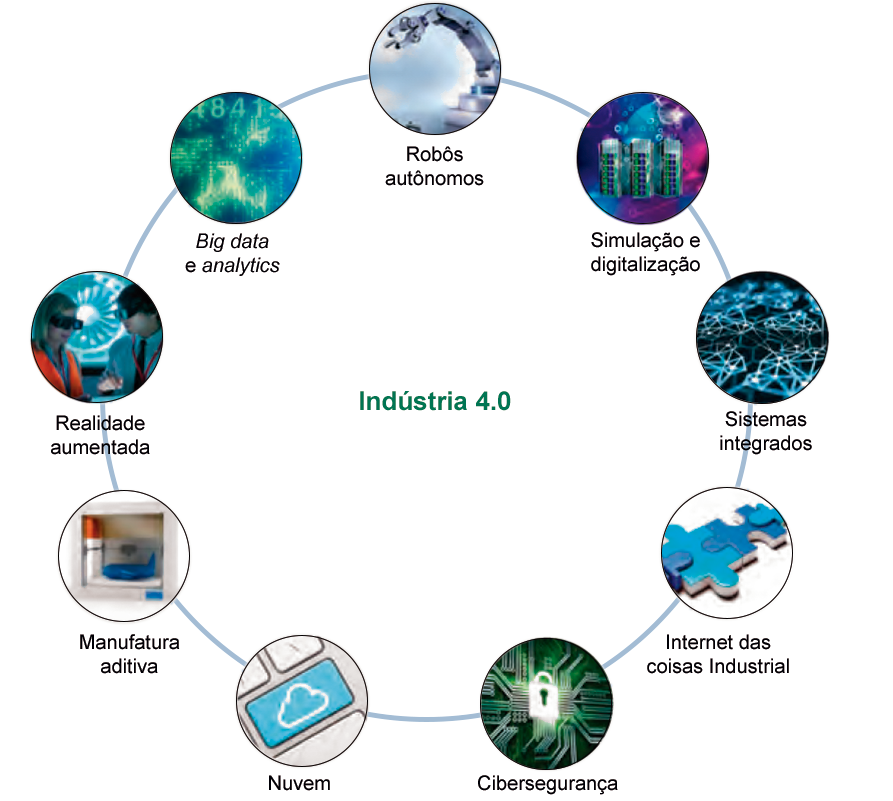
\includegraphics[width=0.8\textwidth]{tecnologias-i4.png}
	\caption{Avanços tecnológicos que moldam a I4.0.}
	\label{fig:tecnologias-i4}
	\fonte{\citeonline{russmann2015industryfour} (adaptado).}
\end{figure}

Após a primeira aparição do termo I4.0 na feira industrial de Hanôver em 2011, o termo ganhou significativa popularidade, principalmente no meio acadêmico e empresarial alemão. O termo foi então incentivado pelo governo alemão \cite{lasi2014industryfour, kagermann2013recommendations}, que apoiou a ideia e anunciou a I4.0 como parte integral da iniciativa estratégica para a indústria alemã, visando liderança em inovação tecnológica \cite{drath2014industrie} como uma abordagem para fortalecer a competitividade de sua indústria manufatureira.

Por meio da iniciativa \textit{Plattform Industrie 4.0}, criada em 2013 pelo Ministério Federal da Educação e Pesquisa (\textit{Bundesministerium für Bildung und Forschung}) \cite{hartmut2019plattform} e com o grupo de trabalho ``Industrie 4.0 Working Group'' em comunicação com diversas associações de engenharia e indústrias alemãs, foram criados documentos oficiais como os de \citeonline{kagermann2013recommendations}, \citeonline{adolph2018roadmap} e \citeonline{bitkom2016implementation}, contendo normas e diretrizes para a implementação da I4.0. Esta iniciativa, atrelada ao entusiasmo acadêmico em torno do projeto I4.0, disseminou o conceito fora da área de língua alemã e popularizou o termo I4.0 no mundo todo como epônimo de um futuro projeto no contexto de indústrias de alta tecnologia.

O impacto econômico dessa revolução industrial traz uma eficiência operacional substancialmente maior, bem como o surgimento de modelos de negócios, serviços e produtos totalmente novos \cite{hermann2016design}.

Em revoluções industriais passadas, os países pioneiros, que se adaptaram às drásticas mudanças de produção, foram os que mais se beneficiaram e se consolidaram como potências econômicas. Embora a mudança completa para a I4.0 possa levar vários anos para ser concretizada \cite{russmann2015industryfour}, os avanços nesta área estabelecem os novos pioneiros e detentores de tecnologias e, portanto, é de interesse de cada país liderar a concorrência global a fim de se consolidar como mercado líder e fornecedor de soluções para a I4.0.

\subsection{Modelo de Arquitetura de Referência para a Indústria 4.0 (RAMI4.0)}
\label{sub:rami4}

O RAMI4.0 é uma representação tridimensional que descreve todos os aspectos cruciais da I4.0. Dessa maneira, inter-relações complexas podem ser divididas em grupos menores e mais simples.

A \autoref{fig:rami4} mostra a representação do RAMI4.0 e a \autoref{tab:rami-eixos} fornece uma descrição detalhada de cada eixo.

\begin{table}[htb]
	\centering
	\footnotesize
	\caption{Eixos do RAMI4.0.}
	\label{tab:rami-eixos}
	\begin{tabular}{p{3cm}p{12cm}}
		\hline
		\textbf{Eixo} & \textbf{Descrição}                                                                                                                                                                                                                                                                                                                                                                                                  \\

		\hline
		Camadas
		              & As seis camadas deste eixo descrevem a decomposição de um ativo em suas funcionalidades, que são cada uma das camadas deste eixo. Esta decomposição do ativo também é chamada de mapeamento virtual. A representação em camadas se origina das TIC, onde as funcionalidades de sistemas complexos são comumente divididas em camadas.                                                                               \\

		\hline
		Ciclo de vida e Cadeia de valor
		              & Este eixo representa o ciclo de vida dos ativos, com base na IEC 62890 para gerenciamento do ciclo de vida. Além disso, é feita uma distinção entre ``tipos'' e ``instâncias''. Um ``tipo'' é criado na fase de desenvolvimento e, uma vez concluída esta fase, esse tipo é liberado para a produção, servindo como modelo para uma ``instância'', que é quando ativo real foi fabricado está operando em produção. \\

		\hline
		Níveis hierárquicos
		              & Neste eixo estão indicados os níveis hierárquicos da IEC 62264, a série de padrões internacionais para sistemas de TI e controle corporativos. Estes níveis representam as diferentes funcionalidades das fábricas. Para representar o ambiente I4.0, as funcionalidades foram expandidas em relação ao padrão internacional ISA-95, incluindo o ``Produto'', o ``Dispositivo de campo'' e o ``Mundo conectado''.   \\
		\hline
	\end{tabular}
\end{table}

A \autoref{fig:eixo-camadas} mostra o detalhamento de cada elemento do eixo ``Camadas'' do RAMI4.0 e sua associação ao modelo completo. O propósito de cada camada, começando da mais inferior (Ativo Técnico) para a mais elevada (Regra de Negócio), é descrito a seguir \cite{bitkom2016implementation}:

\begin{figure}[htb]
	\centering
	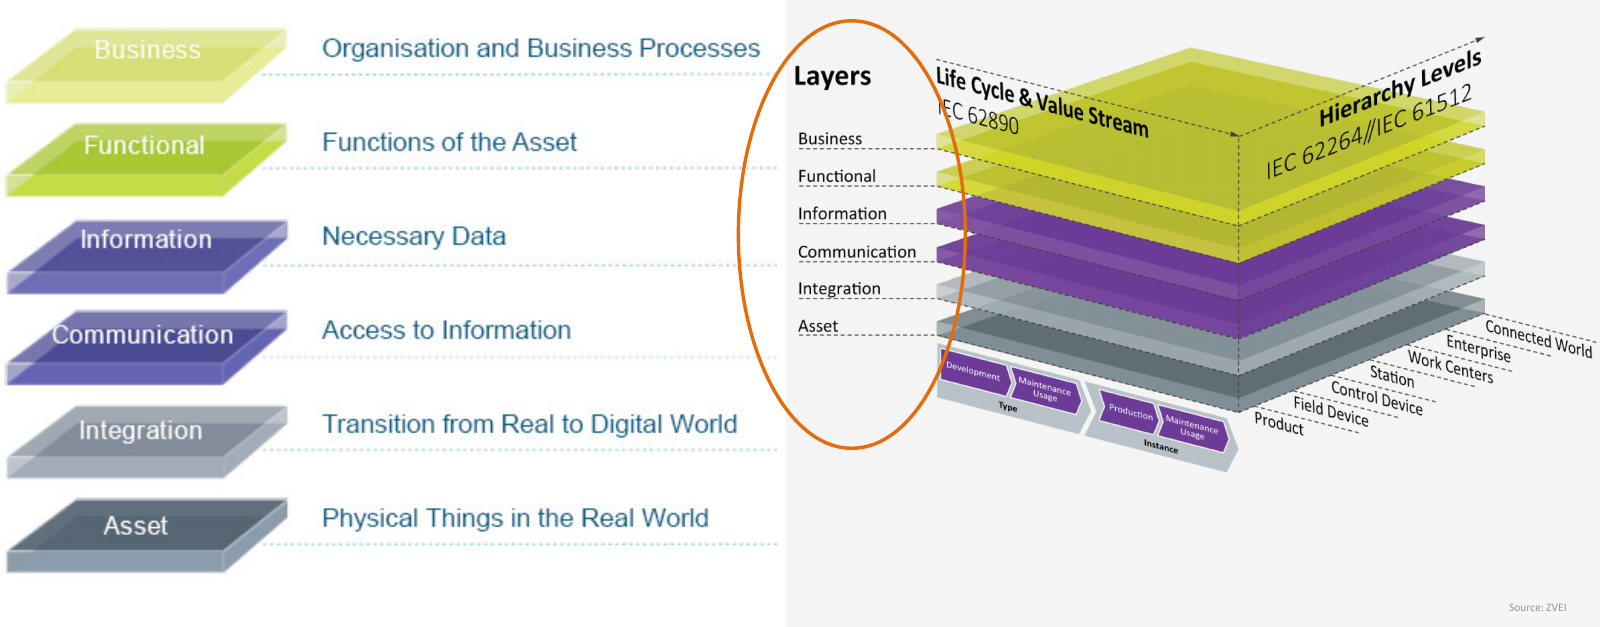
\includegraphics[width=1\textwidth]{eixo-camadas.png}
	\caption{(a) Representação completa do RAMI4.0 e (b) detalhamento do eixo ``Camadas''.}
	\label{fig:eixo-camadas}
	\fonte{\citeonline{gayko2018ramistandardization} (adaptado).}
\end{figure}

\begin{enumerate}
	\item \textbf{Ativo Técnico}: Nesta camada estão os ativos reais, como, por exemplo, uma máquina, um \textit{software}, uma documentação, uma ideia, etc. O trabalhador e seu conhecimento sendo aplicado é também um ativo. Nesta camada estão os fornecedores de dados, ou seja, os elementos que servirão como fonte de dados. Normalmente estes dados gerados pelo ativo são extraído e monitorados para fins de controle da planta de produção;

	\item \textbf{Integração}: Camada responsável pela extração e fornecimento de informações sobre os ativos para as camadas superiores. Representa a digitalização dos ativos. Cada evento no mundo real é refletido também em um evento no mundo digital. Se a realidade mudar, esse evento então é relatado à camada de integração e os dados são atualizados no mundo digital;

	\item \textbf{Comunicação}: Camada responsável pela padronização da interação por meio da adoção de um formato de troca de dados uniforme entre os dispositivos. Esta camada é a responsável pela interoperabilidade entre os ativos na I4.0. Aqui ocorre a integração vertical, ou seja, a interação entre ativos dentro da mesma organização. A camada de Comunicação fornece dados sobre o ativo à camada de informação;

	\item \textbf{Informação}: Camada responsável pelo controle dos dados do ativo. Esta camada agrega todos os dados sobre um determinado ativo e é responsável pelo gerenciamento desses dados. Na camada de informação são garantidos que os dados sejam tratados, pré-processados, armazenados e disponibilizados para os demais ativos do sistema;

	\item \textbf{Funcional}: Camada responsável por manter a descrição formal de todas as funcionalidades do sistema. É também a camada responsável pela integração horizontal de ativos, ou seja, é a porta de interação entre Componentes 4.0 (C4.0) de diferentes organizações. Esta camada é a interface para o fornecimento de informações por meio de serviços para ativos externos à organização;

	\item \textbf{Regra de negócio}: Camada responsável por manter as regras de negócio que o sistema deve seguir como, por exemplo, as condições legais e regulatórias. Esta camada também é responsável por mapear os modelos de negócios e fornecer restrições operacionais da planta de produção.
\end{enumerate}

Já o ordenamento do eixo ``Ciclo de Vida e Cadeia de Valor'' do RAMI4.0 é detalhado na \autoref{fig:eixo-ciclodevida}, juntamente com seu destaque dentro do modelo completo. Este eixo é derivado da norma IEC 62890 \cite{adolphs2015rami}. O seu objetivo é representar o estado de um C4.0 ao longo de toda a sua CS, ou seja, a representação de seu ciclo de vida.

\begin{figure}[htb]
	\centering
	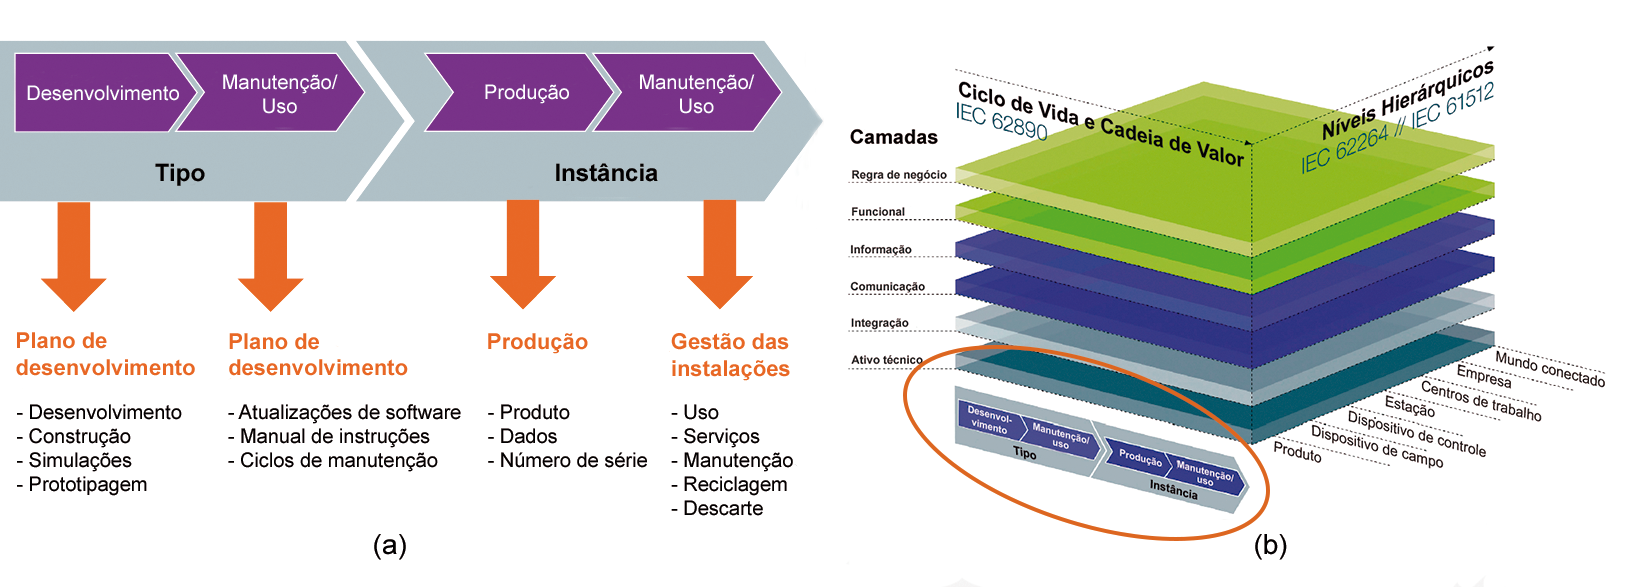
\includegraphics[width=1\textwidth]{eixo-ciclodevida.png}
	\caption{(a) Representação completa do RAMI4.0 e (b) detalhamento do eixo ``Ciclo de Vida e Cadeia de Valor''.}
	\label{fig:eixo-ciclodevida}
	\fonte{\citeonline{gayko2018ramistandardization} (adaptado).}
\end{figure}

Neste eixo é feita a distinção fundamental entre ``tipo'' e ``instância'', cada um correspondendo a uma fase em que o ativo se encontra \cite{adolphs2015rami}.

Um ``tipo'' é sempre criado com uma ideia inicial, ou seja, quando um ativo está na fase de desenvolvimento. Isso abrange o comissionamento, desenvolvimento e testes até a produção inicial de amostras e protótipos \cite{adolph2018roadmap}.

Os ``tipos'' estão presentes desde a concepção/conceitualização até os primeiros protótipos/testes. O ``tipo'' de um ativo é definido por suas propriedades e funcionalidades distintas. Todos os itens que são criados ao longo do projeto de um ativo (e.g., desenhos em CAD, manuais, \textit{softwares}, etc) são incorporados ao ``tipo'' do ativo. Informações externas associadas ao ativo que são criadas ao longo de seu desenvolvimento como informações de \textit{marketing} também são incorporadas ao ``tipo''.

Com a conclusão de todas as etapas de testes e validação, o ``tipo'' é liberado para produção em série. A partir de então, novos ativos podem ser instanciados com base no projeto validado até então.

Com a fabricação do ativo, ``instâncias'' são geradas. Cada ativo fabricado representa uma ``instância'' de um determinado ``tipo'' e assim recebe um número de série exclusivo.

As ``instâncias'' são criadas, produzidas ou fabricadas com base nas informações de um ``tipo'' de ativo. Informações específicas sobre produção, logística, qualidade e testes são associadas à ``instância'' do ativo.

As melhorias sobre um ativo feitas pelo fabricante refletem em um novo ``tipo'', que por sua vez pode ser usado para fabricar novas ``instâncias'', acompanhando, assim, o ciclo de vida deste ativo.

Tanto nas fases ``tipo'' quanto ``instância'', dados de uso e projeto são coletados e associados para então poderem ser armazenados na MDP de cada ativo e serem compartilhados com outros parceiros na CS.

A visão sobre ``tipo'' e ``instância'' apresentada se refere a um ativo como um produto, porém a representação de um ativo é genérica, podendo se aplicar também uma documentação, um processo, uma ideia, etc. Ativos estes que também possuem as respectivas fases referentes ao projeto e operação detalhadas.

O último eixo do RAMI4.0, ``Níveis Hierárquicos'', é apresentado na \autoref{fig:eixo-niveishierarquicos}\textcolor{blue}{a}. Nesta representação, o último nível -- ``Mundo conectado'' (não representado na \autoref{fig:eixo-niveishierarquicos}\textcolor{blue}{b}) -- é a interconexão e interoperabilidade entre diversas organizações, que por sua vez possuem todas as demais camadas inferiores listadas.

\begin{figure}[htb]
	\centering
	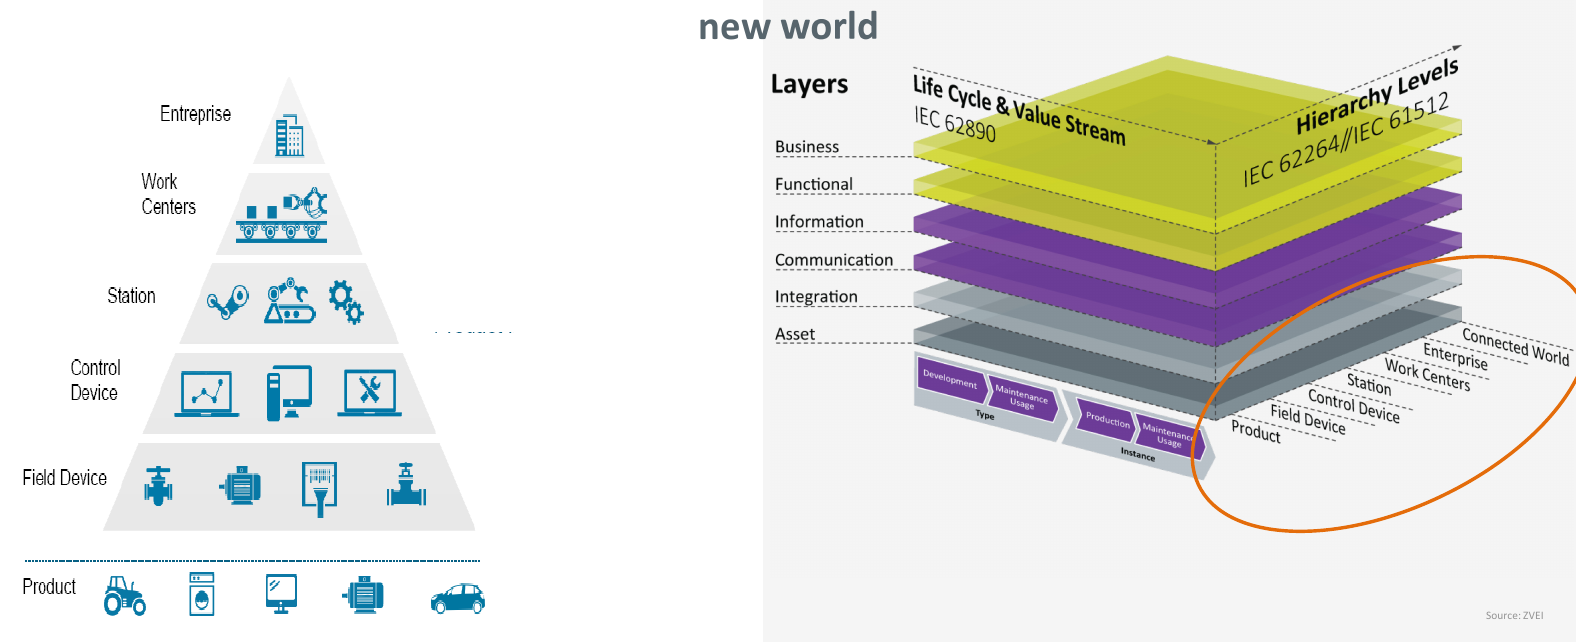
\includegraphics[width=1\textwidth]{eixo-niveishierarquicos.png}
	\caption{(a) Representação completa do RAMI4.0 e (b) detalhamento do eixo ``Níveis Hierárquicos do RAMI4.0''.}
	\label{fig:eixo-niveishierarquicos}
	\fonte{\citeonline{gayko2018ramistandardization} (adaptado).}
\end{figure}

Este eixo é baseado em uma reformulação da IEC 62264, que é a série de padrões internacionais para sistemas de TI e controle corporativos \cite{hankel2015rami}, e faz uma alusão à pirâmide da automação industrial da ISA-95.

Os níveis hierárquicos representam as diferentes funcionalidades das fábricas. Para representar o ambiente I4.0, as funcionalidades foram expandidas além da IEC 62264, que já possui os níveis ``Dispositivo de controle'', ``Estação de trabalho'', ``Centros de trabalho'' e ``Empresa''. Foram adicionados o nível ``Produto'' para descrever funcionalidades de manufatura, o nível ``Dispositivo de campo'' com considerações sobre dispositivos de campo inteligentes, e o nível ``Mundo conectado'' para descrever o grupo de fábricas e a colaboração entre empresas, fornecedores de componentes, consumidores, etc.

\subsection{Asset Administration Shell (AAS)}

Um ativo é qualquer coisa que precise ser conectada para agregar valor a um processo industrial \cite{bader2019aas}, ou seja, tudo que tem valor em um caso de uso específico. Na I4.0, isso pode ser um produto físico, uma peça de equipamento, um \textit{software} ou documentos como plantas, contratos, pedidos, etc.

Na I4.0 cada ativo é encapsulado por um \textit{software} que funciona como uma ``concha'' que administra todos os aspectos relacionados a este ativo. Esta ``concha'' do ativo técnico é denominada \textit{``Asset Administration Shell''} (AAS). O AAS é a representação da parte digital de um ativo no mundo I4.0 \cite{ye2019aas}.

Fazendo uma associação ao eixo ``Camadas'' do RAMI4.0, o AAS engloba as camadas: Regra de Negócio, Funcional, Informação e Comunicação; parte da camada Integração também é contemplada pelo AAS, já que essa é a conexão entre o ativo físico e o meio digital. Tal associação é representada pela \autoref{fig:aas-rami}.

\begin{figure}[htb]
	\centering
	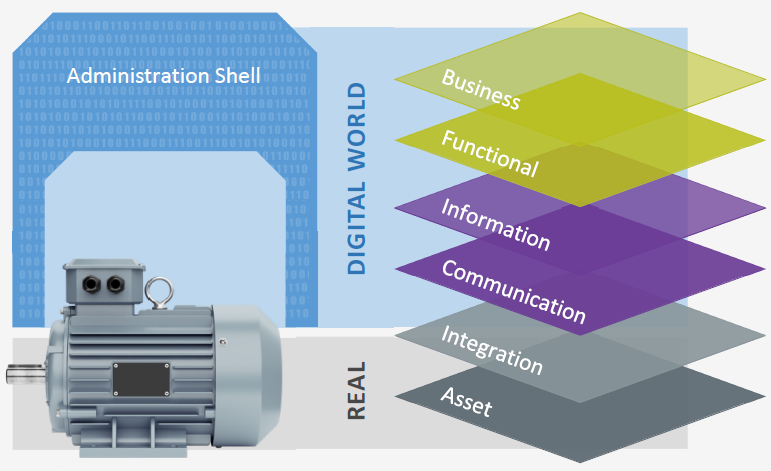
\includegraphics[width=0.8\textwidth]{aas-rami.png}
	\caption{Representação do AAS.}
	\label{fig:aas-rami}
	\fonte{\citeonline{gayko2018ramistandardization} (adaptado).}
\end{figure}

O AAS consiste em vários submodelos nos quais são descritas todas as informações e funcionalidades de um determinado ativo, incluindo suas características, propriedades, condições, parâmetros, dados de medições e capacidades \cite{bader2019aas}. A \autoref{fig:aas-submodelos} exemplifica um AAS contendo informações relevantes do ativo em forma de ``submodelos''.

\begin{figure}[htb]
	\centering
	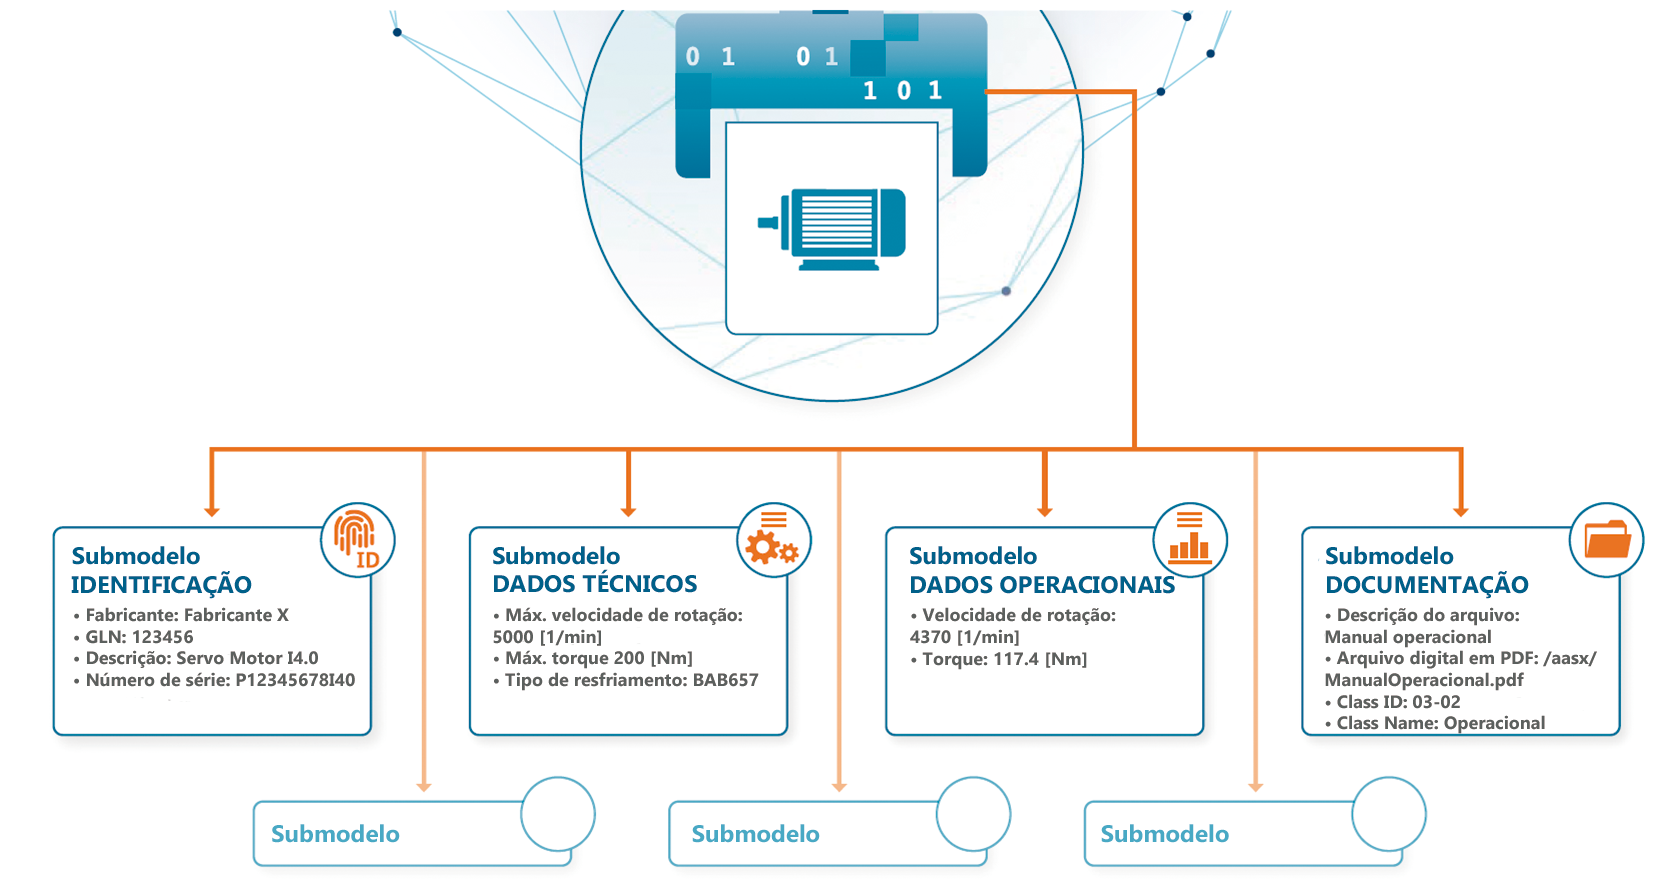
\includegraphics[width=1\textwidth]{aas-submodelos.png}
	\caption{Exemplificação de um AAS para um servomotor, incluindo os submodelos de identificação, dados técnicos, dados operacionais e documentação.}
	\label{fig:aas-submodelos}
	\fonte{\citeonline{bader2019aas} (adaptado).}
\end{figure}

Os submodelos são unidades básicas de organização dentro de um AAS que agregam informações semelhantes. Eles são divididos em dois tipos: submodelos básicos e submodelos livres \cite{bader2019aasimplementation}.

Os submodelos básicos são unidades de organização que se aplicam a muitos ou todos os ativos dentro do mundo I4.0. Já os submodelos livres são acordados entre os parceiros na CS e possuem um uso específico para um determinado ativo.

O AAS é um elo entre os ativos reais e seus correspondentes digitais no mundo conectado. Dentro da I4.0, os ativos possuem um AAS com capacidade de comunicação com outros dispositivos \cite{bader2019aas}. O conjunto Ativo-AAS é denominado ``Componente I4.0'' (C4.0).

%A \autoref{fig:aas-conexao} ilustra a interação entre diferentes C4.0 em um ambiente de manufatura.

%\begin{figure}[htb]
%	\centering
%	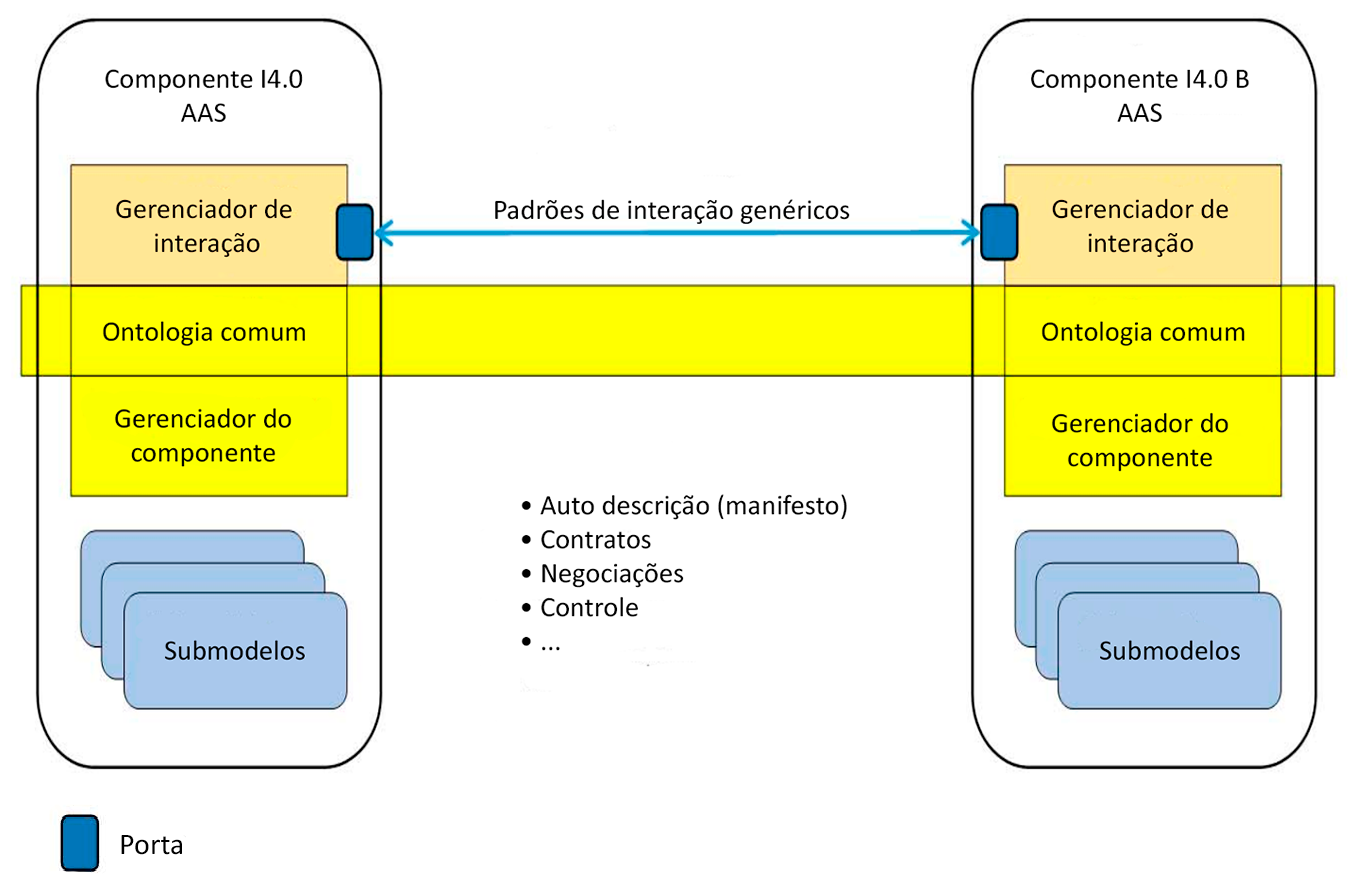
\includegraphics[width=1\textwidth]{aas-conexao.png}
%	\caption{Exemplo de comunicação entre diferentes C4.0.}
%	\label{fig:aas-conexao}
%	\fonte{\citeonline{marcon2018asset} (adaptado).}
%\end{figure}

A integração dos ativos, representada pelos C4.0, em um nível funcional requer uma descrição padronizada das funções (ou capacidades) dos ativos em questão. A padronização de submodelos para descrever detalhadamente cada função pode ser usada para definir requisitos para a fabricação de produtos \cite{bedenbender2017aasexamples}. A \autoref{fig:submodelos} mostra um exemplo de detalhamento de funções de um ativo para o caso de diferentes tipos de processos de fabricação.

\begin{figure}[htb]
	\centering
	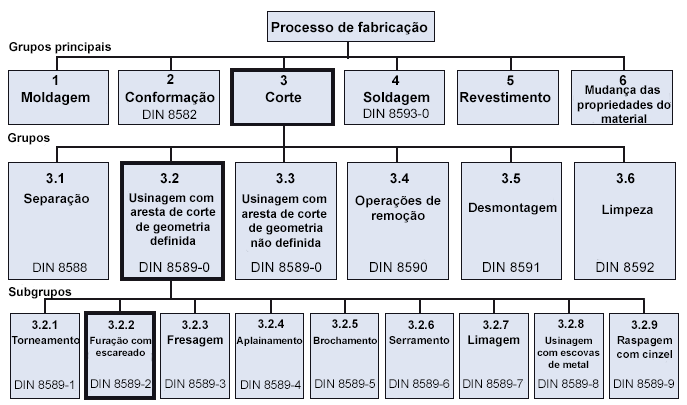
\includegraphics[width=1\textwidth]{submodelos.png}
	\caption{Exemplo de processos de fabricação de um ativo (uma máquina) detalhados por meio de submodelos.}
	\label{fig:submodelos}
	\fonte{\citeonline{bedenbender2017aasexamples} (adaptado).}
\end{figure}

No ambiente de manufatura baseado na I4.0, o produto descreve os requisitos necessários para a sua fabricação, e então esses requisitos são comparados com as descrições das funções dos ativos disponíveis para o fabricar. Portanto, a seleção de um ativo é otimizada, baseando-se nos requisitos do próprio produto (ativo requisitante) e nas descrições das funções dos ativos disponíveis para a manufatura.

Desta forma, um C4.0 tem todas as informações para a efetiva interoperabilidade entre ativos no mundo conectado, inclusive os seus próprios requisitos, suas regras de negócio, limitações técnicas e todas as demais características que se relacionem ao ativo e sua interação com o ambiente.

\section{Logística \& Cadeia de Suprimentos (CS)}
\label{sec:logistica}

A logística é o processo de planejamento, implantação e controle do fluxo de mercadorias, serviços e informações desde o ponto de origem até o ponto de consumo de forma eficiente e eficaz com o propósito de atender às exigências dos clientes \cite{cscmp2013supplychainglossary}. Essa definição sugere a logística como um processo, o que significa que inclui todas as atividades importantes para a disponibilização de bens e serviços aos consumidores quando e onde estes quiserem adquiri-los \cite{ballou2006cadeiasuprimentos}.

A logística é a essência do comércio \cite{ballou2006cadeiasuprimentos}, ela contribui para que pessoas não mais sejam obrigadas a viver perto das fontes de produção e possam trocar informações e mercadorias com outras regiões de forma efetiva, contribuindo decisivamente para melhorar o padrão econômico de vida geral.

O intercâmbio de informações é um tema chave da logística moderna. Este nicho é chamado de logística da informação e lida com o fluxo de informações entre humanos e/ou máquinas dentro ou entre organizações \cite{haftor2011information}, que se agrupam formando uma rede de criação de valor por meio de informações. A Logística da Informação é intrinsecamente relacionada a processos de gestão da informação e tecnologias de informação.

A CS, por outro lado, é um conceito mais amplo. A CS é onde a logística é exercida. São as partes necessárias para dar suporte ao pedido de um cliente, desde o produtor até o consumidor final. A gestão da CS tem como alvo a orquestração de todas as partes envolvidas, criando assim uma logística integrada como forma de otimizar ao máximo o processo de fornecimento de um produto, serviço ou informação.

Uma CS simples envolve fornecedor, produtor e cliente \cite{hugos2018supplychain}, porém conceitos modernos estendem a noção de uma CS, passando a incluir diversos outros fornecedores de serviços em áreas como logística, finanças, \textit{marketing} e desenvolvimento, que, mediante coordenação e colaboração, criam oportunidades para redução de custos e melhoria dos serviços fornecidos ao consumidor. A \autoref{fig:cadeia-de-suprimentos} exemplifica a inter-relação das partes em uma CS estendida.

\begin{figure}[htb]
	\centering
	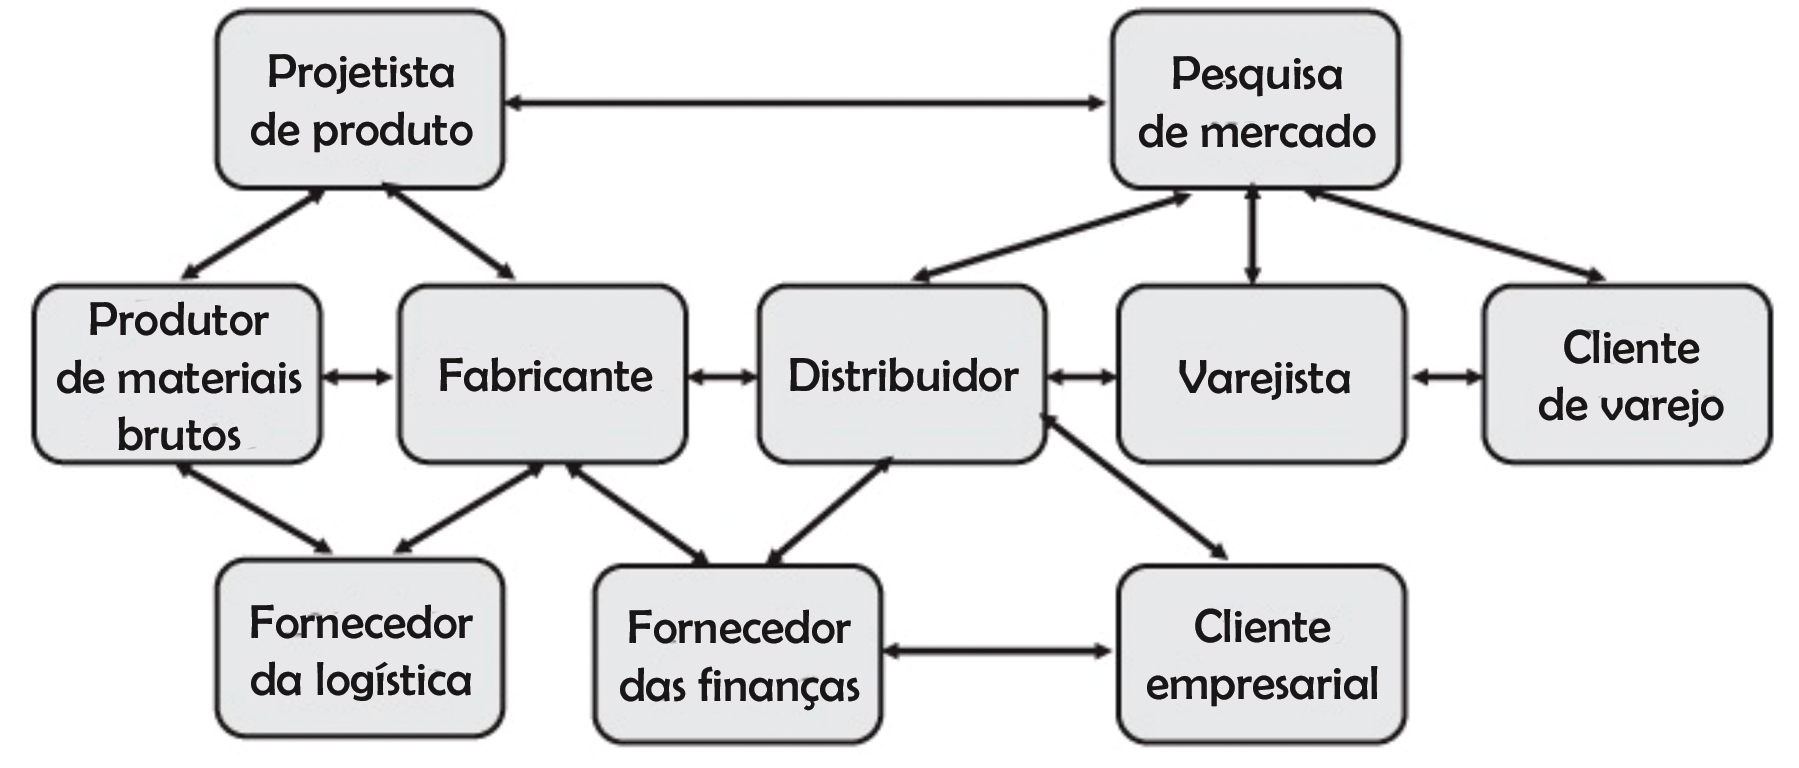
\includegraphics[width=1\textwidth]{cadeia-de-suprimentos.png}
	\caption{Exemplo de CS estendida.}
	\label{fig:cadeia-de-suprimentos}
	\fonte{\citeonline{hugos2018supplychain} (adaptado).}
\end{figure}

Além do eficiente fluxo de materiais e produtos dentro da CS, é imprescindível a manutenção de um canal para troca de informações entre as partes, pois sem uma comunicação adequada, gerentes podem tomar decisões supostamente racionais, porém que afetam negativamente outras partes da cadeia, como o efeito chicote \cite{lee1997bullwhip}, que é a distorção da percepção da procura de um produto que vai se ampliando ao longo da CS. Erros de comunicação desse tipo podem acarretar problemas como o aumento do custo de transporte, o elevado tempo de aprovisionamento ao cliente e o desgaste no relacionamento com os fornecedores.

Ao longo da CS pode-se observar processos que agregam valor ao produto em desenvolvimento. As etapas de transformação do produto com adição de valor ao longo da CS define o que se chama de Cadeia de Valor (CV).

Uma CV é um conjunto de atividades que organizações de um setor específico desempenham a fim de entregar um produto ou serviço que tenha algum valor perceptível para o mercado \cite{porter1985competitiveadvantage}. A ideia da CV é baseada na agregação de valor ao produto a cada processo de transformação ocorrido, processo esse que envolve a aquisição e consumo de recursos (mão de obra, materiais, equipamentos, instalações, administração, etc). As atividades em uma CV são divididas em duas categorias: as atividades primárias e as atividades de apoio \cite{porter1985competitiveadvantage} (vide \autoref{fig:porter-cadeia-de-valor}).

\begin{figure}[htb]
	\centering
	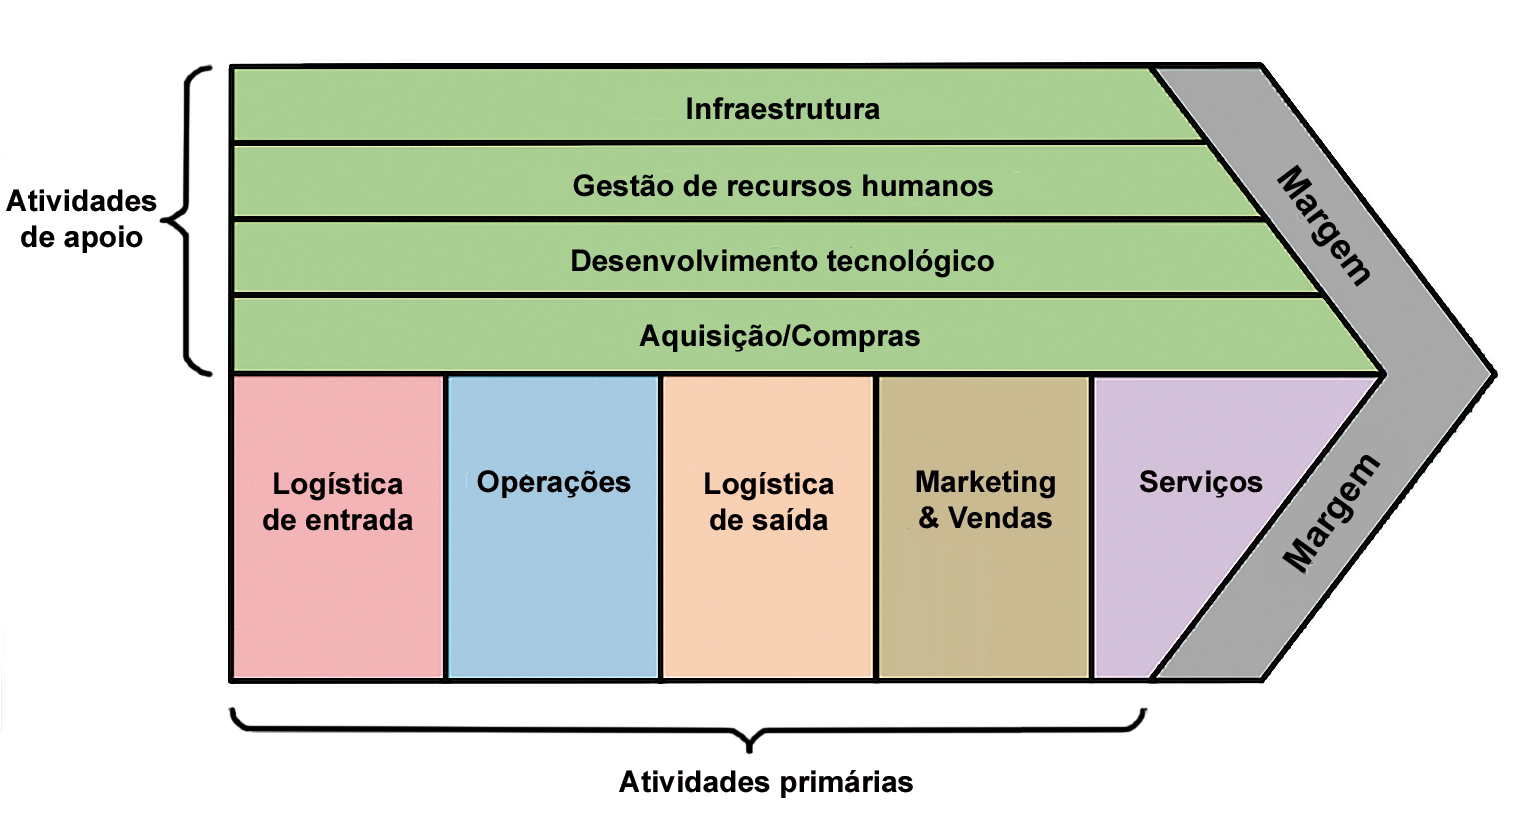
\includegraphics[width=1\textwidth]{porter-cadeia-de-valor.png}
	\caption{Cadeia de valor de Porter.}
	\label{fig:porter-cadeia-de-valor}
	\fonte{\citeonline{porter1985competitiveadvantage} (adaptado).}
\end{figure}

As CV estão focadas em fornecer o máximo valor ao cliente (valor perceptível) com o menor custo e, portanto, é um indicador de competitividade. Com o crescente acirramento da competição, essas devem procurar novas formas de agregar mais valor perceptível aos seus produtos, sendo isto em forma de redução de preço, aumento de qualidade, suporte, ou qualquer outra nova funcionalidade.

Outra forma de agregação de valor está no princípio de valor compartilhado, que envolve a geração de valor econômico de forma a criar também valor para a sociedade como um todo \cite{porter2011valorcompartilhado}, com o enfrentamento de suas necessidades e desafios. Soluções que visem o aumento das condições de trabalho, a maior racionalidade e eficiência no tratamento dos recursos naturais necessários para sua atividade e outras formas de balancear o \textit{trade-off} entre eficiência econômica e progresso social são estratégias para se recuperar a legitimidade e a percepção de valor pela sociedade da atividade empresarial.

\subsection{Logística 4.0}

Com o entusiasmo sobre o tema I4.0 surgido a partir de 2011, surgiram diversas linhas de pesquisa relacionadas. Uma dessas vertentes é relacionada aos novos desafios tecnológicos na logística e por vezes é denominada ``Logística 4.0''. Estes novos desafios tecnológicos estão relacionados primariamente ao intenso uso das Tecnologias de Informação e Comunicação (TIC) e de Internet das Coisas Industrial (IIoT) \cite{barreto2017industry}.

A inserção dessas novas tecnologias ao escopo de estudo da logística acarreta em novos desafios como a necessidade de transparência dos processos (visibilidade ao longo da CS) e o controle de integridade (produtos certos, no tempo, lugar, quantidade, condição e preço certos) \cite{barreto2017industry}.

As CS atuais podem ser extremamente grandes e complexas (alta interdependência entre as partes) e, portanto, sem uma correta gestão, podem levar à tomada de decisões não ótimas por parte dos gestores. Por estes aspectos, as CS podem se aproveitar da nova forma de organização da I4.0 (ou da Logística 4.0), tornando os processos cada vez mais automatizados a fim de se atender os novos requisitos da sociedade moderna.

Dentro da CS, identificadores individuais podem ser usados a fim de se implementar a conectividade de objetos e informações requeridas no contexto da I4.0. Neste sentido, um exemplo de tecnologia relacionada a identificação de itens é o RFID (\textit{Radio-Frequency IDentification}), que permite criar uma identificação única para um ativo. Outra forma de identificação única é o endereço MAC (\textit{Media Access Control}) em interfaces de rede para comunicação de dispositivos em rede, sendo essencial para o tráfego de dados na Internet. A utilização de identificadores é essencial para aplicações de conceitos de I4.0 \cite{alyahya2016rfidwarehousing, vlachos2014rfidimpact, fan2015inventory, bibi2017rfidfood}, pois possibilita a troca autônoma de informações.

A troca de informações ao longo da CS é uma das variáveis que influenciam na eficiência da cadeia \cite{barreto2017industry}, especialmente em CS complexas e com alta interdependência entre as partes. O estudo sobre formas e processos visando a troca de informações é, portanto, um tema relevante dentro da Logística 4.0 e também foco de estudo neste trabalho.

A Logística 4.0, portanto, estabelece uma série de paradigmas que organizações atuando no ramo logístico deverão seguir nos próximos anos para se manterem competitivas. Conceitos de operação como o intercâmbio de informações instantâneas, soluções automatizadas e análise de dados em tempo real abrem caminhos para novos modelos de negócios \cite{strandhagen2017logistics}, que se tornarão essenciais na eficiência em logística moderna.

\section{Ciclo de vida do produto}
\label{sec:ciclo-de-vida}

Dentro da I4.0, os ativos dizem respeito a equipamentos, produtos, máquinas, peças, pessoas e quaisquer outros elementos envolvidos no ambiente industrial. Neste trabalho são abordados os ativos que se deslocam pela CS, isto é, os produtos. Estes produtos, conforme são fabricados e deslocam por cada elo da cadeia, produzem informações sobre logística, operações, fabricação, etc. Pode-se dizer que estas informações são geradas e compartilhadas ao longo de sua existência, ou seja, ao longo de seu ciclo de vida. Portanto, neste trabalho é analisado o ciclo de vida de um tipo particular de ativo, que é o produto que percorre a CS.

O conceito de ciclo de vida do produto foi elaborado em meados da década de 1960 com o propósito de criar um modelo que fosse capaz de explicar o sucesso ou fracasso de um produto introduzido no mercado, sendo capaz também de identificar momentos certos para modificar estratégias de preço, fabricação e quando o produto deve ser descontinuado \cite{cao2012lifecycle}. O modelo inicialmente desenvolvido por \citeonline{levitt1965lifecycle} mostra o padrão de produtos na história passando por quatro estágios bem definidos: desenvolvimento de mercado, crescimento, maturidade e declínio, conforme observado na \autoref{fig:product-life-cycle}.

\begin{figure}[htb]
	\centering
	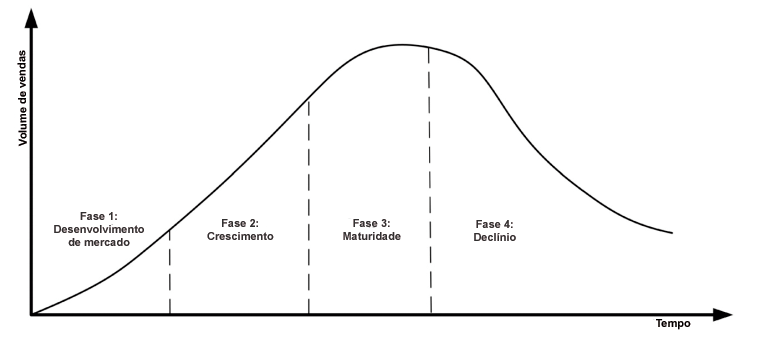
\includegraphics[width=1\textwidth]{product-life-cycle.png}
	\caption{Estágios do ciclo de vida do produto.}
	\label{fig:product-life-cycle}
	\fonte{\citeonline{levitt1965lifecycle} (adaptado).}
\end{figure}

Vista a tendência global de redução do ciclo de vida do produto devida a rápida taxa de introdução de novas tecnologias para satisfazer a demanda dos clientes, especialmente no mercado de produtos eletrônicos \cite{trappey2008lifecycle}, novas versões de modelos de ciclo de vida do produto vêm sendo elaboradas considerando outros aspectos de mercado e não somente sob a visão da área de \textit{Marketing}. Alguns estudos \cite{cao2012lifecycle} envolvendo ciclo de vida levam em consideração fatores não abordados nos modelos originais como, por exemplo, a fase de pesquisa e desenvolvimento, a retroalimentação de dados, assim como o descarte e reciclagem do produto.

A \autoref{fig:ciclo-de-vida-extensao} mostra um modelo de ciclo de vida do produto com elementos que incluem a fase de desenvolvimento e a renovação do produto. A renovação do produto e a decorrente extensão de sua vida é essencial, pois mantém o produto no mercado na forma de novas versões e, assim, amplia as receitas mediante ações estratégicas para agregação de valor. O modelo do ciclo de vida e os elementos presentes sempre irão variar conforme a natureza do produto e tipo de mercado consumidor onde o mesmo está inserido.

\begin{figure}[htb]
	\centering
	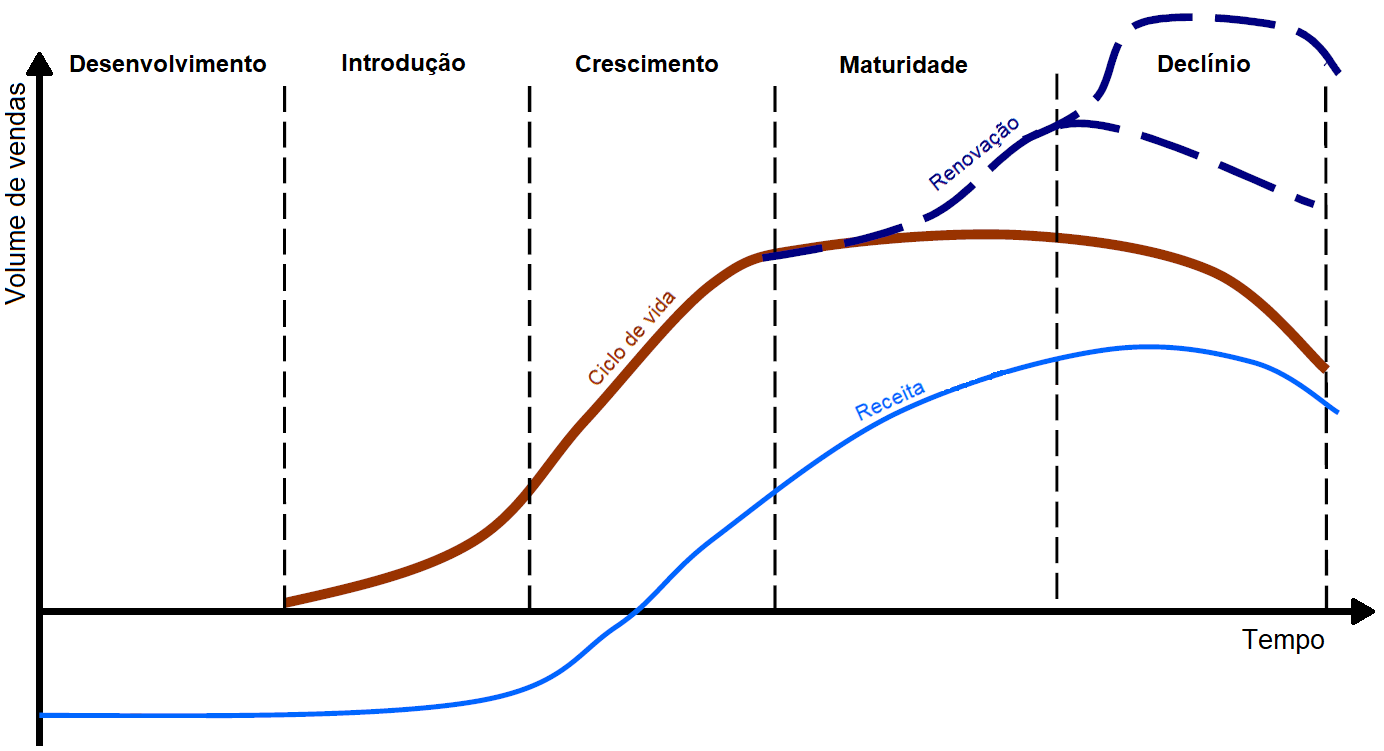
\includegraphics[width=0.9\textwidth]{ciclo-de-vida-extensao.png}
	\caption{Modelo de ciclo de vida do produto com renovação do produto.}
	\label{fig:ciclo-de-vida-extensao}
	\fonte{\citeonline{liu2010marketingrisk} (adaptado).}
\end{figure}

A gestão do ciclo de vida do produto (GCVP) refere-se ao gerenciamento de um ativo ao longo dos estágios típicos de sua vida útil (vide \autoref{fig:product-life-cycle}). Esta gestão dentro dos estágios mencionados pode se referir, por exemplo, à fabricação, comercialização, uso ou qualquer outra fase do ciclo de vida em que o produto se encontra.

A GCVP tem como finalidade auxiliar gestores na tomada de decisões de negócios por meio de estratégias como políticas de preços, expansão de mercado, retirada do produto ou inserção de novas versões, etc. A função da GCVP não é gerenciar apenas um produto, mas gerenciar de maneira integrada todas as partes, assim como o portfólio de produtos de uma organização \cite{stark2015lifecycle}.

Em nível mais alto, o objetivo do GCVP é aumentar as receitas do produto, reduzir custos relacionados a ele, maximizar o valor do portfólio e maximizar o valor dos produtos atuais e futuros para clientes e acionistas \cite{stark2015lifecycle}.

Mais recentemente, novas propostas de modificações de processos industriais por meio da GCVP aparecem como formas de se agregar mais valor ao produto considerando os ciclos de vida cada vez mais curtos. A Logística 4.0 surge com nova forma de abordagem da gestão do ciclo de vida do produto, considerando as mais novas necessidades do produto e de seus respectivos consumidores.

\section{Memória digital do produto (MDP)}
\label{sec:mdp}

O termo MDP surgiu pela primeira vez em 2007 por meio de um boletim de notícias de tecnologia de uma empresa alemã fabricante de conectores elétricos e eletrônicos \cite{wahlster2007digitalmemory}. À época, o termo foi tratado com analogia a um diário, que mantinha todas as informações do produto ao longo de seu ciclo de vida.

Em outras referências, este conceito se relaciona a sistemas que permitem a coleta de dados em todas as fases do ciclo de vida do produto para a distribuição e/ou análise \cite{brandherm2011productmemory,blume2014mdp}. Os dados de interesse do produto são heterogêneos e podem ser gerados e/ou consumidos por diferentes elos ao longo de sua CS. A \autoref{fig:mdp} ilustra este comportamento.

\begin{figure}[htb]
	\centering
	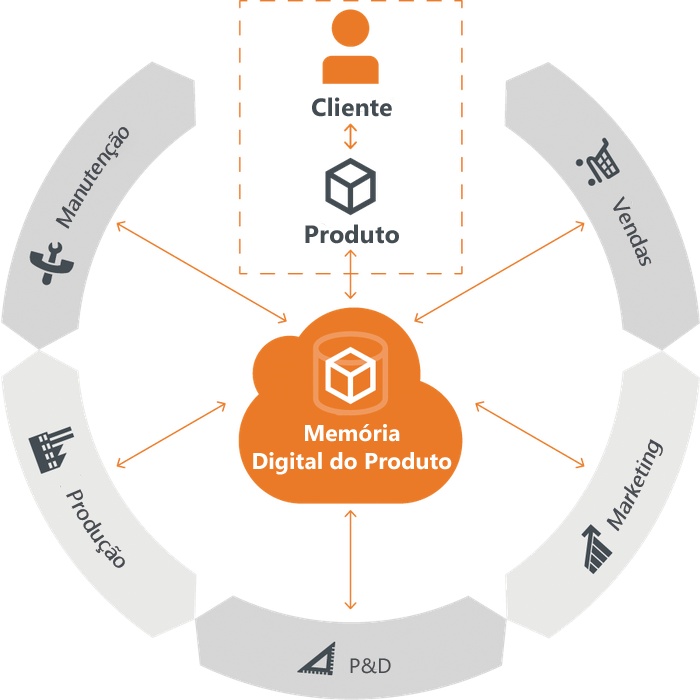
\includegraphics[width=0.8\textwidth]{mdp}
	\caption{Coleta de dados do produto ao longo da CS.}
	\label{fig:mdp}
\end{figure}

Sua relevância está no fato da tendência de produtos novos apresentarem ciclos de vida cada vez mais curtos, e também devido ao fato das CS serem compostas por redes cada vez mais complexas, com múltiplos fornecedores e clientes. Com isso, a MDP manteria registros digitais dos produtos, permitiria o monitoramento de seu estado atual e o rastreamento de sua posição dentro do processo produtivo. Segundo \citeonline{wahlster2007digitalmemory}, o acesso a essas informações pelas partes interessadas seria de vital importância na competitividade de organizações produtoras e de comércio, além de abrir novas proteções em relação à pirataria.

O conceito de MDP pode ser introduzido nos produtos no cenário de I4.0 e por meio dela extrair e armazenar informações relevantes de eventos ocorridos ao longo do ciclo de vida do produto a fim de fornecer serviços a todo o ambiente com o qual o produto se relaciona \cite{brandherm2011productmemory}. A MDP fornece também uma forma de rastreabilidade, uma vez que pode armazenar informações geoespaciais do ativo ao longo do tempo.

O armazenamento de informações sobre o produto ao longo de sua CS é importante, pois torna possível acessar e utilizar informações do mundo real provenientes de diferentes fontes para o potencial benefício das partes interessadas naquele produto \cite{brandherm2011productmemory}, como, por exemplo, fabricantes, transportadores, varejistas e consumidores. Ela também é relevante no pós-venda, onde a MDP continua a ser disponibilizada e ativa, dando a possibilidade ao consumidor de ainda manter contato com cada elo da CS e se beneficiar de serviços individuais que se acumulam na memória \cite{brandherm2011productmemory}.

\section{Arquitetura orientada a serviços (SOA)}
\label{sec:soa}

Arquitetura Orientada a Serviços (\textit{Service Oriented Architecture} - SOA) é uma forma de conceber e implementar um sistema em que serviços são disponibilizados a outros sistemas por meio de um protocolo de comunicação comum em uma rede de computadores \cite{bell2008soa}. Um serviço é uma unidade de funcionalidade que pode ser fornecida/acessada remotamente. A SOA se destina a ser independente de fornecedores, produtos e tecnologias.

Para quem consome um serviço, a abordagem é como uma caixa preta, o que significa que o consumidor não sabe ou não precisa estar ciente do funcionamento interno deste serviço, sendo relevante apenas as interfaces de entrada e saída, definidas em um documento de contrato, acordado pelo fornecedor e pelo consumidor do serviço. Os serviços representam uma lógica de fornecimento de resultados. É uma abstração de problemas, ou seja, toda a complexidade interna inerente aos serviços pode ser abstraída pelos consumidores dos serviços.

SOA é uma abordagem que traz novas perspectivas uma vez que se estabelece um conjunto de princípios para a construção de um sistema autônomo e interoperável \cite{candido2009soa}. SOA tem por objetivo aumentar a eficiência, agilidade e produtividade de um sistema por meio da adoção generalizada do conceito de serviços \cite{souit2013soa}. Dentro do mundo da I4.0 e de sistemas produtivos estes princípios também podem ser aplicados.

Os serviços dentro do ambiente de manufatura encapsulam as funcionalidades necessárias, ocultando todas as heterogeneidades das partes do sistema, assegurando, desta forma, características de flexibilidade, confiabilidade e fácil implementação de	soluções \cite{groba2008soa}.

A SOA dentro do meio industrial pode ser implementada por meio de um \textit{middleware}, que é um \textit{software} que integra os diferentes aplicativos em um sistema. A \autoref{fig:middleware} ilustra como se dá a interconexão entre ativos em um sistema (a) sem e (b) com um \textit{middleware}.

\begin{figure}[htb]
	\centering
	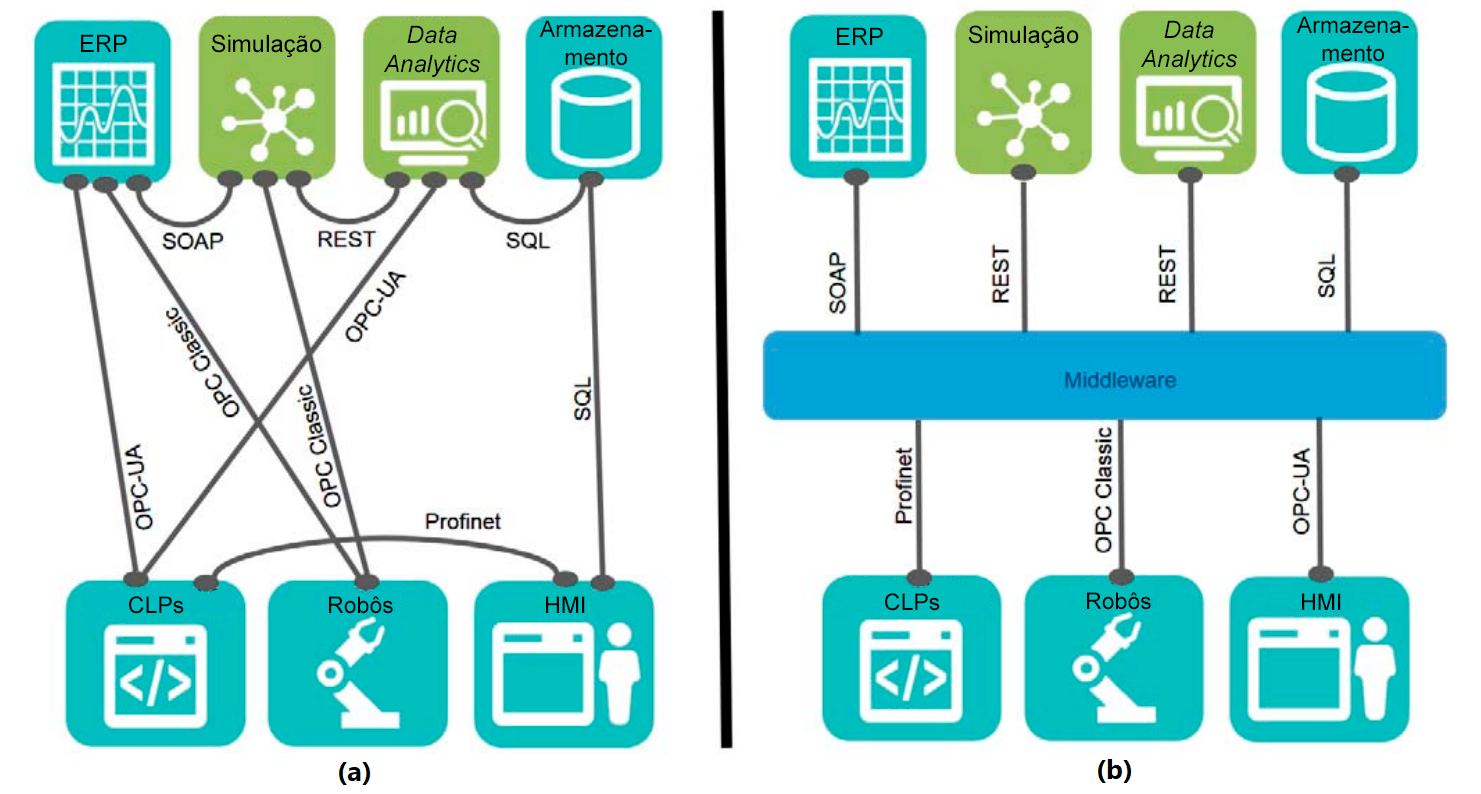
\includegraphics[width=0.9\textwidth]{middleware.png}
	\caption{Comunicação entre ativos em um sistema (a) sem \textit{middleware} e (b) com \textit{middleware}.}
	\label{fig:middleware}
	\fonte{\citeonline{gosewehr2017middleware} (adaptado).}
\end{figure}

SOA está relacionada à ideia de uma Interface de Programação de Aplicação (\textit{Application Programming Interface} - API), que é o conjunto de rotinas e padrões estabelecidos por um \textit{software} para a utilização das suas funcionalidades por aplicativos externos.

Para se disponibilizar um serviço por meio de uma API, o conceito de \textit{Web Services} (WS) é vastamente utilizado \cite{souit2013soa}, pois assim é possível fornecer serviços utilizando a Internet (protocolos TCP/IP) como meio de tráfego de informações.

\subsection{Web Services (WS)}
\label{sub:web-services}

Um WS é uma interface que descreve uma série de operações acessíveis por meio de uma linguagem de descrição de serviços padronizada \cite{gottschalk2002webservices}. Um WS executa uma tarefa específica ou um conjunto de tarefas e retorna ao usuário o resultado da operação. Cada aplicação servidora de serviços pode ter a sua própria linguagem, que é traduzida para uma linguagem de transferência comum, como o XML (\textit{Extensible Markup Language}), JSON (\textit{JavaScript Object Notation}) e outros.

Por meio de WS, as aplicações podem ser descritas, publicadas, localizadas e invocadas em uma rede de comunicação tipo WWW (\textit{World Wide Web}) \cite{souit2013soa}. Para que os WS sejam fornecidos e consumidos, é necessária uma interface de comunicação entre as duas partes. Em sistemas automatizados esta interface é uma API (\textit{Application Programming Interface}), pela qual sistemas programáveis podem se comunicar. Um padrão comumente utilizado é a API REST, que é detalhada na \autoref{sub:rest}.

O WS envolve três atores básicos: o provedor de serviços, o repositório de serviços e o solicitante de serviços; e por três operações básicas: a publicação, a procura e a interação \cite{gottschalk2002webservices}. A \autoref{fig:webservice-componentes} ilustra os atores e a interação entre eles por meio das operações.

\begin{figure}[htb]
	\centering
	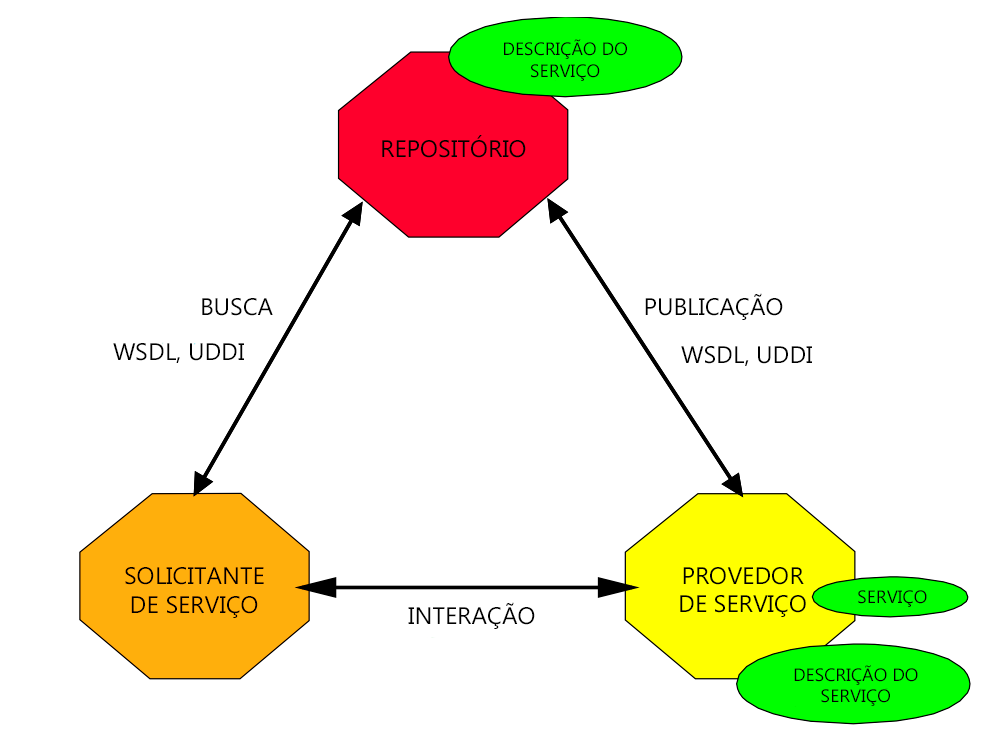
\includegraphics[width=0.8\textwidth]{webservice-componentes}
	\caption{Componentes de um WS e operações.}
	\label{fig:webservice-componentes}
	\fonte{\citeonline{kreger2001webservices} (adaptado).}
\end{figure}

Detalhadamente, os atores em um WS são:

\begin{itemize}
	\item \textbf{Provedor de serviços}: Entidade que hospeda e fornece um determinado serviço. Esta entidade permite que clientes solicitem serviços e recebam suas respectivas respostas. O provedor de serviços é responsável também por fornecer uma descrição sobre o serviço prestado e publicar esta descrição em um repositório acessível ao solicitante;

	\item \textbf{Repositório de serviços}: Entidade que armazena e fornece a descrição sobre diversos WS. Os WS são descobertos pelo solicitante, por meio do repositório, para que assim possa decidir o serviço que melhor o atenda;

	\item \textbf{Solicitante de serviços}: Entidade que requer um determinado serviço e solicita a sua execução. O solicitante de serviço pode ser uma pessoa acessando pelo navegador ou uma outra aplicação realizando solicitações por meio de API.
\end{itemize}

Já as operações básicas em WS são:

\begin{itemize}
	\item \textbf{Publicação}: Publicação da descrição do serviço pelo provedor em um repositório para que o serviço se torne acessível ao público e os solicitantes possam localizá-lo;

	\item \textbf{Busca}: Busca e recebimento da descrição de um serviço. O solicitante pode receber a descrição do serviço pelo provedor ou por meio do repositório;

	\item \textbf{Interação}: Comunicação direta entre solicitante e provedor para o fornecimento de serviços. Nesta fase, o solicitante se decide por um determinado serviço dentre os disponíveis no repositório e inicia uma interação com o provedor por meio de uma API.
\end{itemize}

As etapas de interação entre as entidades (cliente e servidor) são representadas por meio do diagrama da \autoref{fig:uml-webservice}.

\begin{figure}[htb]
	\centering
	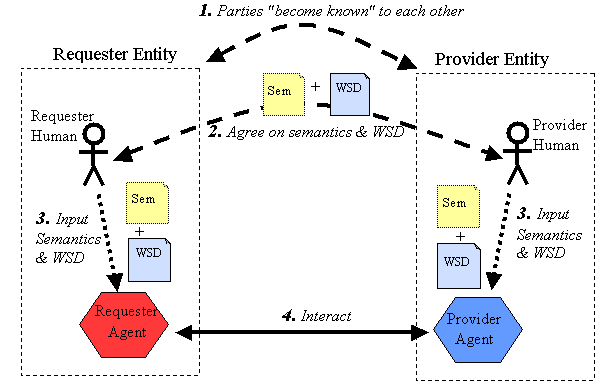
\includegraphics[width=1\textwidth]{uml-webservice}
	\caption{Diagrama com os atores e interações em um WS.}
	\label{fig:uml-webservice}
	\fonte{\citeonline{booth2004webservice} (adaptado).}
\end{figure}

Neste diagrama, a semântica e a descrição do WS (\textit{Web Service Description} -- WSD) representam os documentos com os quais ambas as partes devem concordar para que haja o efetivo fornecimento e consumo do serviço.

O WSD define os formatos de mensagem, tipos de dados, protocolos de transporte e formatos de troca de dados que devem ser usados entre o solicitante e o provedor \cite{booth2004webservice}. O WSD representa um acordo que rege a mecânica de interação com esse serviço.

Já a semântica de um WS é o documento que determina o comportamento esperado de resposta deste serviço, pode ser explícito ou implícito, oral ou escrito, processável por máquina ou orientado a humanos, e pode ser um acordo legal ou um acordo informal \cite{booth2004webservice}.

Os WS se tornaram atrativos, pois podem ser implementados com as tecnologias HTTP e XML, que estão disponíveis na maioria dos navegadores de internet e possuem suporte nativo em diversas linguagens de programação. A disponibilização de serviços interativos na \textit{Internet} se tornou popular e com isso surgem novos modelos de negócios como o SaaS (\textit{Software as a Service}), PaaS (\textit{Platform as a Service}), IaaS (\textit{Infrastructure as a Service}) e até mesmo MaaS (\textit{Manufacturing as a Service}) \cite{annunziata2019maas, nichols2020maas, siepen2019maas}.

Dentro da I4.0 não é diferente. O \autoref{cha:arquitetura} descreve como os ativos podem publicar suas funcionalidades em repositórios e executarem determinadas tarefas mediante solicitação por parte do consumidor.

\subsection{Transferência Representacional de Estado (REST)}
\label{sub:rest}

A Transferência Representacional de Estado (\textit{Representational State Transfer} - REST) define padrões para acesso e disponibilização de WS. Os WS que seguem o padrão REST são denominados \textit{RESTful Services} \cite{fielding2000rest}.

O REST possibilita a interoperabilidade entre sistemas na \textit{Internet}, pois permite que os sistemas solicitantes acessem e manipulem representações textuais de recursos usando um conjunto uniforme e predefinido de operações \cite{booth2004webservice}.

O REST veio gradualmente substituindo o padrão SOAP (\textit{Simple Object Access Protocol}). Hoje, REST é comumente utilizado para o compartilhamento de informações em novos WS, sendo o padrão SOAP usado em sistemas legado \cite{serrano2014soaplegacy}. Apesar de ambos os padrões serem baseados no HTTP e HTTPS, o REST geralmente contém um \textit{payload} de mensagem mais leve por trafegar dados no formato JSON (\textit{JavaScript Object Notation}), ao contrário do padrão SOAP que utiliza o formato XML (\textit{eXtensible Markup Language}).

O REST estabelece as orientações e boas práticas de uma interface que devem ser satisfeitas para que possa ser referida como um serviço \textit{RESTful}. Esses princípios são \cite{fielding2000rest}:

\begin{enumerate}
	\item \textbf{Cliente-Servidor}: segregação das interfaces dos usuário das interfaces do banco de dados. Desta forma, padroniza-se a interface para a interação com um banco de dados, trazendo mais portabilidade e flexibilidade aos sistemas e melhorando a sua escalabilidade;

	\item \textbf{Sem estado}: um estado é o conjunto de dados salvos no servidor durante uma interação entre dois sistemas. Portanto uma interação sem estado significa que para o servidor cada nova mensagem é equivalente a uma interação com um cliente novo, uma vez que não há informações salvas sobre as interações anteriores. Com isso, cada solicitação do cliente ao servidor deve conter todas as informações necessárias para o servidor processar a solicitação. Desta forma, a solicitação não pode depender de qualquer tipo de contexto a ser armazenado no servidor, o estado da sessão é mantido inteiramente no cliente;

	\item \textbf{Cache}: respostas para as solicitações podem ser armazenadas em memória (\textit{cache}). Quando a resposta puder ser armazenada em \textit{cache}, o cliente poderá reutilizar a resposta já recebida anteriormente e evitar de se realizar uma nova requisição;

	\item \textbf{Interface uniforme}: As interfaces são padronizadas entre os sistemas que se comunicam por meio de um serviço REST. São definidas para os serviços REST quatro restrições de interface: identificação de recursos, manipulação de recursos por meio de representações; mensagens auto descritivas e hipermídia como forma de interação com a aplicação;

	\item \textbf{Sistema em camadas}: o sistema é organizado em camadas hierárquicas, restringindo, assim, o comportamento do componente de forma que cada um possa ter acesso somente às camadas imediatas (acima ou abaixo) com as quais está interagindo;
\end{enumerate}

O principal item de manipulação relacionado a um serviço REST é o recurso. Um recurso é qualquer informação a ser manipulada: documento, imagem, uma coleção de objetos, etc. Os serviços REST utilizam um identificador único de um recurso como forma de referência em consultas. Já as coleções são conjuntos de recursos de uma mesma categoria, como por exemplo uma  lista de usuários cadastrados, a lista de comentários em uma publicação, etc.

Cada método do protocolo HTTP está relacionado a um tipo de operação no REST. A \autoref{tab:methods-rest} mostra as possíveis operações e seus métodos HTTP correspondentes.

\begin{table}[htb]
	\centering
	\caption{Mapeamento dos métodos HTTP em um serviço \textit{RESTful}.}
	\label{tab:methods-rest}
	\begin{tabular}{p{3.5cm}p{2cm}p{9cm}}
		\hline
		\textbf{Método HTTP} &
		\textbf{Escopo}      &
		\textbf{Semântica}                                   \\[5mm]

		\hline
		GET                  &
		Coleção              &
		Retorna uma coleção com todos os recursos.           \\[5mm]

		\hline
		GET                  &
		Recurso              &
		Retorna um único recurso.                            \\[5mm]

		\hline
		POST                 &
		Coleção              &
		Cria um novo recurso em uma coleção.                 \\[5mm]

		\hline
		PUT                  &
		Recurso              &
		Atualiza um recurso completamente.                   \\[5mm]

		\hline
		PATCH                &
		Recurso              &
		Atualiza um recurso parcialmente.                    \\[5mm]

		\hline
		DELETE               &
		Recurso              &
		Exclui um recurso da base de dados.                  \\[5mm]

		\hline
		OPTIONS              &
		Recurso              &
		Retorna os métodos HTTP disponíveis e outras opções. \\[5mm]

		\hline
	\end{tabular}
	\fonte{\citeonline{fielding2000rest} (adaptado).}
\end{table}

Tanto para uma API REST quanto para uma API SOAP, é necessária a definição de um contrato, que é a sua documentação. Este documento descreve o comportamento esperado da API, o que inclui as URLs dos \textit{endpoints} (rotas), os métodos de cada rota, argumentos e exemplos de chamadas (\textit{requests}) com suas respectivas respostas \cite{santos2020apicontract}. O contrato garante ao cliente que o servidor responderá em um formato específico, evitando erros e exceções no cliente por quebra de esquema.

Existem vários formatos de arquivo que permitem criar um contrato e obter sua documentação. O mais comumente utilizado para a documentação de API REST é o OpenAPI \cite{santos2020openapi}, anteriormente conhecido como \textit{Swagger}.

Para as API SOAP, o WSDL (\textit{Web Service Description Language}) é utilizado como contrato \cite{booth2004webservice}. As API com outros protocolos de comunicação, como por exemplo o RPC (\textit{Remote Call Procedure}), suportam o contrato por meio de arquivos protobuf (\textit{protocol buffers}).

O contrato é definido pelos provedores do serviço e destinado aos consumidores da API, ou seja, às organizações e desenvolvedores que irão utilizá-la. O documento geralmente é criado pela própria equipe de desenvolvimento que elabora o serviço.

\section{Modelagem de sistemas}
\label{sec:modelagem-de-sistemas}

Sistema é um conjunto de elementos interdependentes de modo a formar um todo organizado. Também pode ser entendido como um conjunto de órgãos funcionais, entidades ou partes e as relações entre eles, com um objetivo geral a ser atingido \cite{mulbert2005sistemas}.

No contexto da Logística 4.0, um sistema pode ser definido como o conjunto de diferentes CS ligadas por meio de relacionamentos interorganizacionais, que fazem acontecer os fluxos envolvidos (de dinheiro, materiais, bens e informações) \cite{oliveira2016supplychain}.

As técnicas de modelagem e análise de sistemas na CS são meios de promover a sua melhoria como um todo. A utilização destas técnicas auxiliam no entendimento sobre o comportamento do sistema e dos relacionamentos entre suas partes. Auxiliam também na reprodução e análise de diferentes cenários e soluções, na previsibilidade de possíveis perturbações de mercado e na melhoria nos processos de distribuição.

Com a intensificação da globalização é cada vez mais comum a criação de CS complexas, envolvendo várias organizações dispersas geograficamente. Por isso, as ferramentas de suporte à tomada de decisões são utilizadas para auxiliar no sentido de fornecer soluções mais adequadas à dinâmica de diversas CS. A modelagem e análise auxiliam na tomada de decisões e são úteis no entendimento das interações da CS e sobre como melhorar o seu desempenho \cite{oliveira2016supplychain}.

Um desafio para o desenvolvimento de bons modelos nessa área é a adoção de metodologias claras que possam facilitar e agilizar o processo de se realizar a modelagem e a análise de aspectos da CS. Uma metodologia apresenta um direcionamento sobre os procedimentos a serem tomados a fim de se atingir um objetivo, porém cada problema a ser analisado requer especificações diferentes, o que demanda adaptações dos procedimentos originais.

\citeonline{miyagi1996controle} define os sistemas feitos pelo homem (\textit{man-made systems}), como sistemas de manufatura, transporte, comunicação, redes de computadores, etc. Estes sistemas são caracterizados por uma dinâmica decorrente da ocorrência de eventos que geram a alteração discreta de estados e, portanto, são classificados como Sistemas a Eventos Discretos (SED). Um SED é uma classificação de sistemas de acordo com seu comportamento, determinado pela ocorrência de eventos que alteram de forma discreta e instantânea o estado do sistema.

Para a modelagem de SEDs, a aplicação de ferramentas como a Rede de Petri e suas variações como \textit{Production Flow Schema} (PFS) são formas de auxílio no desenvolvimento de sistemas de controle e automação.

A utilização da técnica de PFS no contexto da I4.0 auxilia no mapeamento das operações e interações entre as partes do sistema, uma vez que a dinâmica de interação pode ser classificada com um SED. Neste trabalho o PFS é utilizado a fim de se indicar as atividades relacionadas à CS de um produto e as mapear para as camadas do RAMI4.0.

\subsection{Production Flow Schema (PFS)}

O PFS é uma técnica indicada para nível conceitual de modelagem, análise e controle de SEDs \cite{miyagi1996controle}.

No PFS, são identificadas as atividades, que por sua vez podem incluir vários outros eventos e estados organizados hierarquicamente.

Por meio de modelos em PFS é possível especificar uma estrutura de processos assim como da arquitetura de um sistema, indicando as interações entre as partes desse sistema. Além disso, com o PFS, os fluxos e as atividades podem ser descritos de forma desacoplada de qualquer tecnologia necessária para a implementação do sistema \cite{pisching2018equipmentrami}.

Qualquer processo produtivo representado em PFS apresentará os seguintes elementos estruturais:

\begin{itemize}
	\item Atividades: representação dos componentes ativos;
	\item Distribuidores: representação dos componentes passivos;
	\item Arcos orientados: representação das relações entre os componentes ativos  e passivos.
\end{itemize}

A \autoref{fig:pfs-elementos} descreve os elementos do PFS e sua representação gráfica.

\begin{figure}[htb]
	\centering
	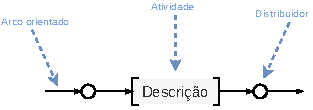
\includegraphics[width=0.9\textwidth]{pfs-elementos}
	\caption{Elementos do PFS.}
	\label{fig:pfs-elementos}
	\fonte{\citeonline{pisching2018pfs} (adaptado).}
\end{figure}

A atividade corresponde à realização de certas unidades ou conjuntos de operações como, por exemplo, um processamento, uma montagem, desmontagem, etc. Os distribuidores correspondem aos lugares de entrada e saída de itens materiais como, por exemplo, um \textit{buffer} de entrada ou saída de peças ou de itens relativos à informações. Já os arcos orientados indicam a direção dos fluxos e a relação entre os elementos do sistema.

Os arcos conectando a parte externa das atividades (conectados diretamente nos colchetes) indicam um fluxo principal (primário) (\autoref{fig:pfs-fluxos}\textcolor{blue}{a}); já os arcos conectando a parte interna da atividade indicam um fluxo secundário (\autoref{fig:pfs-fluxos}\textcolor{blue}{b}) \cite{miyagi1996controle}.

Um terceiro tipo de arco é usado para representar a interface direta entre atividades e é indicado por meio de um arco conectando diretamente a parte interna de duas atividades (\autoref{fig:pfs-fluxos}\textcolor{blue}{c}). Este arco indicador de interação direta entre atividades é usado neste trabalho para modelar interações entre diferentes níveis, como operações de solicitação e resposta \cite{pisching2018pfs}.

\begin{figure}[htb]
	\centering
	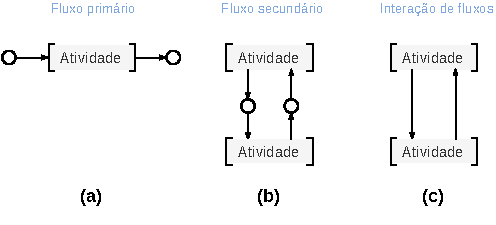
\includegraphics[width=1\textwidth]{pfs-fluxos}
	\caption{Tipos de fluxo no PFS.}
	\label{fig:pfs-fluxos}
	\fonte{\citeonline{pisching2018pfs} (adaptado).}
\end{figure}

Os fluxos de processo do sistema em PFS são modelados por meio de uma abordagem \textit{top-down}, assim os resultados podem ser refinados sucessivamente, detalhando, a cada iteração, a atividade representada. A modelagem do sistema em PFS, portanto, parte de um alto nível de abstração, seguido de sucessivos detalhamentos que resultam em modelos em rede de Petri e que por sua vez podem ser utilizados para a análise dinâmica dos processos do sistema.

Desta forma, o PFS é uma linguagem de alto nível independente de tecnologia e de fabricantes para modelar os processos do sistema. A relevância de se adotar uma linguagem como o PFS para a representação de sistemas está na padronização da comunicação com especialistas de diferentes áreas, como arquitetos, engenheiros e desenhistas \cite{pisching2018pfs}. Assim, há uma efetiva comunicação sobre a interação entre as partes de um sistema e sobre os fluxos de itens materiais e/ou de informação em diferentes níveis do sistema em análise, como, por exemplo, produtos, ordens de serviço, comandos para máquinas, informações de sensores, etc.
